% =============================================================
%  Left-shunt unified power quality conditioner: the model ls_upqc
%  (pwr-control/left-shunt-unified-power-quality-conditioner, folder ls_upqc, branch dev)
%  pwr-control documentation - compile with pdflatex (three times) from inside this folder:
%      pdflatex upqc.tex && pdflatex upqc.tex && pdflatex upqc.tex
%  The single-line diagram, the control diagrams and the DAB power curve are drawn in this file (TikZ,
%  pgfplots). The figures of Section 7 and their numbers come from two simulations of the default case of
%  init_model.m (with and without the storage, logging step 25 us): py/upqc_summary.m (MATLAB) writes the
%  summaries py/data/*.csv (ignored by the repository) and *_numbers.txt from the results, py/upqc_figures.py
%  draws the figures:
%      cd py && python3 upqc_figures.py ../figures
% =============================================================
\documentclass[11pt,a4paper]{scrartcl}
% ===================== PACKAGES =====================
\usepackage[british]{babel}
\usepackage[tmargin=1in, bmargin=1in, lmargin=0.75in, rmargin=0.75in]{geometry}
\usepackage[dvipsnames,table]{xcolor}  % prima di tikz, listings, ecc.

\usepackage{tikz}
\usepackage{graphicx}
\usepackage{pgfplots}
\pgfplotsset{width=12cm, compat=1.9}
\usepackage{setspace}
\usepackage{chemmacros}
\usepackage{chemfig}
\usepackage{esint}
\usepackage{tabularray}
\usepackage{makeidx}
\usepackage{epstopdf}
\usepackage{amssymb}
\usepackage{mathrsfs}
\usepackage{bm}
\usepackage{amsmath}
\usepackage{enumitem}
\usepackage[english]{varioref}
\usepackage{lipsum}
\usepackage{fancyhdr}
\usepackage{float}
\usepackage{empheq}
\usepackage[framemethod=tikz]{mdframed}
\numberwithin{equation}{section}
\usepackage{eso-pic}
\usepackage{calc}
\usepackage{nccmath}
\usepackage{caption}
\usepackage{subcaption}
\usepackage{gensymb}
\usepackage{amsfonts, amsthm, epsfig, epstopdf, titling, url, array}
\usepackage{tabularx}
\usepackage{makecell}
\usepackage{booktabs}
\usepackage{array}
\usepackage{siunitx}
\sisetup{input-digits=0123456789\pi}
\usepackage[symbol]{footmisc}
\usepackage{multicol}
\usepackage{boondox-cal}
\usepackage{blindtext}
\usepackage{changepage}
\usepackage{nomencl}
\usepackage{hyperref}
\usepackage{xurl}
\usepackage{ragged2e}
\usepackage[version=4]{mhchem}  % ← conflitto di opzioni
\usepackage{longtable}
\usepackage{chemformula}
\usetikzlibrary{arrows.meta,positioning,calc}

% ===================== SI UNITS =====================
\DeclareSIUnit\atm{atm}
\DeclareSIUnit{\var}{var}
\DeclareSIUnit{\pu}{p.u.}


% ===================== MATH OPERATORS =====================
\DeclareMathOperator{\rank}{rank}
\DeclareMathOperator{\atantwo}{atan2}
\DeclareMathOperator{\spn}{span}

% ===================== COMMANDS =====================
\newcommand{\abs}[1]{\left|#1\right|}
\newcommand{\sign}{\text{sign}}
\newcommand{\centered}[1]{\begin{tabular}{@{}l@{}} #1 \end{tabular}}

% ===================== COLORS =====================
\definecolor{mycolor1}{rgb}{0.97, 0.97, 0.97}
\definecolor{mycolor2}{rgb}{0.97, 0.97, 0.97}
\definecolor{tableShade}{gray}{0.9}

% ===================== THEOREM ENVIRONMENTS =====================
\theoremstyle{it}
\newtheorem{defn}{Definition}[section]
\newtheorem{assumption}{Assumption}[section]
\newtheorem{thm}{Theorem}[section]
\newtheorem{lemma}{Lemma}[section]
\newtheorem{corollary}{Corollary}[section]
\theoremstyle{definition}
\newtheorem{example}{Example}[section]

% ===================== CUSTOM ENVIRONMENTS =====================
\newenvironment{myitemize_1}{
	\begin{itemize}[topsep=0pt]
		\setlength{\topsep}{2pt}
		\setlength{\itemsep}{2pt}
		\setlength{\parskip}{2pt}
		\setlength{\parsep}{2pt}
	}{\end{itemize}}

\newmdenv[
innerlinewidth=0.5pt,
roundcorner=4pt,
backgroundcolor=mycolor2,
linecolor=mycolor1,
innerleftmargin=6pt,
innerrightmargin=6pt,
innertopmargin=6pt,
innerbottommargin=6pt
]{mybox}

% ===================== TABLE COLUMN TYPES =====================
\newcolumntype{Y}{>{\hsize=2\hsize}X}
\newcolumntype{Z}{>{\centering\arraybackslash\hsize=0.857\hsize}X}

% ===================== SECTION DEPTH =====================
\setcounter{secnumdepth}{3}
\setcounter{tocdepth}{3}

% ===================== PAGE STYLE =====================
\setlength{\headheight}{20pt}
\setlength{\headsep}{20pt}

\pagestyle{fancy}
\fancypagestyle{firstpage}{\rhead{}}
\fancyhead[L]{\slshape\nouppercase{\leftmark}}
\chead{}
\rhead{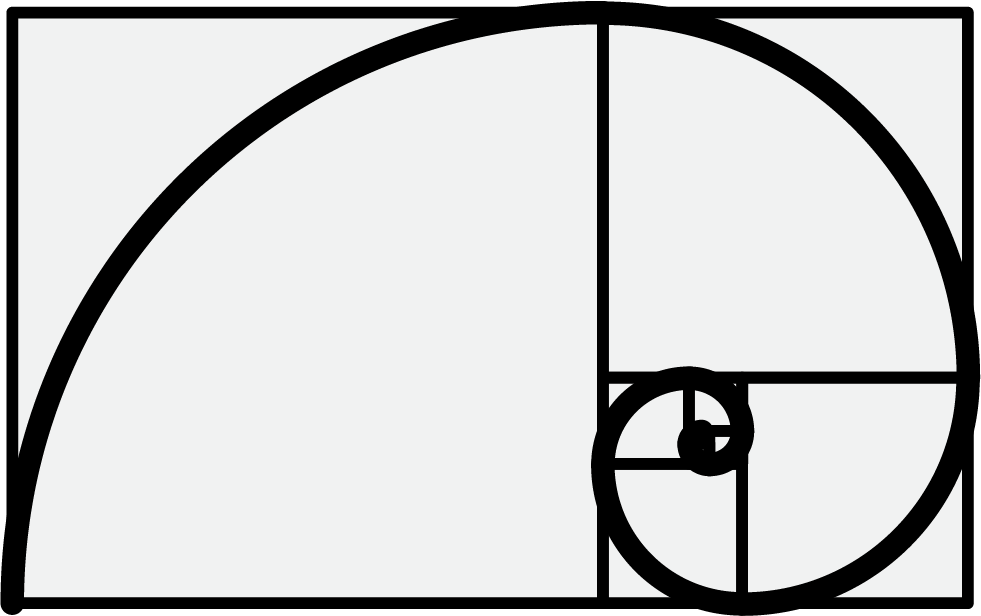
\includegraphics[height=0.75cm]{../../AAA_template_latex_settings/pwr-control_logo_doc.png}}
\lfoot{\href{http://www.pwr-control.com}{pwr-control.com}}
\cfoot{-\ \thepage\ -}
\rfoot{\textit{}}
\renewcommand{\headrulewidth}{0.4pt}
\renewcommand{\footrulewidth}{0.4pt}


\geometry{
	a4paper,
	top    = 2.5cm,
	bottom = 3.0cm,
	left   = 2.5cm,
	right  = 2.5cm
}

\hypersetup{
	colorlinks = true,
	urlcolor   = blue,
	linkcolor  = black,
	citecolor  = black
}

\pagenumbering{gobble}

\usetikzlibrary{shapes.geometric,fit,decorations.pathreplacing}
\pgfplotsset{compat=1.16}

\newcommand{\ped}[1]{_{\mathrm{#1}}}
\newcommand{\code}[1]{\texttt{#1}}
\newcommand{\pun}{\,\mathrm{pu}}
\newcommand{\jj}{\mathrm{j}}
\renewcommand{\tabularxcolumn}[1]{>{\raggedright\arraybackslash}p{#1}}
\setlength{\emergencystretch}{3em}
\sisetup{per-mode=symbol}
\DeclareSIUnit{\VA}{VA}
\DeclareSIUnit{\var}{var}

% ---------------- document metadata (read by the title page) ----------------
\newcommand{\DocCategory}{Technical Note}
\newcommand{\DocField}{Power Electronics and Control Systems}

\newcommand{\DocTitle}{%
	{\fontsize{20}{24}\selectfont\bfseries Left-shunt unified power quality conditioner\par}
	\vspace{14pt}
	{\fontsize{16}{23}\selectfont\bfseries the model \code{ls\_upqc}:\\ shunt active filter, voltage stabilizer,\\ dual active bridge and battery on a \SI{690}{V} grid\par}
}

\newcommand{\DocSubtitle}{%
	Description and user guide of the Simulink/Simscape model \code{ls\_upqc} of \code{pwr-control/left-shunt-unified-power-quality-conditioner} after the revision of November 2026: the system, the structure of the model and its clocks, the control of the three converters, the parameters, how to run it, the results of the default case and the open points.
}

\newcommand{\DocAuthor}{Davide Bagnara}
\newcommand{\DocRevision}{00}
\newcommand{\DocDate}{November 2026}

\newcommand{\DocAbstract}{%
	The model \code{ls\_upqc} simulates a left-shunt unified power quality conditioner on a \SI{690}{V}, \SI{50}{Hz} grid: a \SI{250}{\kilo\watt} shunt active filter (SAF) facing the grid, a \SI{250}{\kilo\watt} voltage stabilizer (VS) that injects a voltage in series with a \SI{433}{\kilo\watt} load through three single-phase transformers, and an optional \SI{250}{\kilo\watt} dual active bridge (DAB) with a \SI{1200}{V} lithium-ion battery on their common DC link. This note describes the model after the revision of November 2026, which made it run with the MATLAB Home licence (fewer than \num{1000} nonvirtual blocks), replaced the setup functions of the library with one parameter struct and local functions, fixed the power stage of the DAB, the start-up and the case without the storage, and renamed the blocks after the acronyms \code{saf}, \code{vs} and \code{dab}. It covers the system and its data, the structure and the clocks of the model, the control of the three converters, the parameters, how to run the model and post-process its results, and the simulation of the default fault ride-through test (an asymmetric dip to \SI{0.40}{pu} of positive sequence) with and without the storage, where the energy balance of the DC link decides the behaviour. It also corrects the control of the DAB, whose DC-link voltage loop could drive the phase shift beyond the top of the power curve and was too slow for the step of power at the start of a dip: with the storage the DC link now stays within \SI{2}{\percent} of \SI{1200}{V} through the dip and the load voltage at \SI{1.00}{pu}; without the storage the SAF cannot bring from the faulted grid the power that the VS needs, the DC link falls to \SI{686}{V} and the system has not recovered at the end of the simulation. The open points close the note.
}

\newcommand{\RevisionHistory}{%
	00 & November 2026 & First issue (the folder had only the skeleton of the document): the model \code{ls\_upqc} after the revision of November 2026 (init with one \code{param} struct and local functions, model within the \num{1000} nonvirtual blocks of the MATLAB Home licence, fixes of the DAB and of the start-up, labels \code{saf}, \code{vs}, \code{dab}); simulations of the default case with and without the storage. & \DocAuthor \\
}

\newcommand{\MetaLabelA}{Project Repository}
\newcommand{\MetaValueAUrl}{https://github.com/pwr-control/left-shunt-unified-power-quality-conditioner/tree/dev/ls_upqc}
\newcommand{\MetaValueALabel}{left-shunt-unified-power-quality-conditioner.git (ls\_upqc)}

\newcommand{\MetaLabelB}{Framework}
\newcommand{\MetaValueB}{MATLAB/Simulink/Simscape, Python}

\begin{document}

% =============================================================
%  pwr-control LaTeX template - FRONTESPIZIO
%
%  Da richiamare come prima istruzione dopo \begin{document}:
%      % =============================================================
%  pwr-control LaTeX template - FRONTESPIZIO
%
%  Da richiamare come prima istruzione dopo \begin{document}:
%      % =============================================================
%  pwr-control LaTeX template - FRONTESPIZIO
%
%  Da richiamare come prima istruzione dopo \begin{document}:
%      \input{../../AAA_template_latex_settings/titlepage}
%
%  Il documento deve definire prima di \begin{document}:
%      \DocCategory   categoria del documento
%      \DocField      area tecnica
%      \DocTitle      titolo (una o due righe)
%      \DocSubtitle   sottotitolo
%      \DocAuthor     autore/i, separati da virgola
%      \DocRevision   numero di revisione corrente (es. 00)
%      \DocDate       data della revisione corrente
%      \DocAbstract   abstract
%      \RevisionHistory  righe della tabella di revisione, nel formato
%                        Rev. & Date & Description & Authors \\
%      \MetaLabelA \MetaValueAUrl \MetaValueALabel
%      \MetaLabelB \MetaValueB
% =============================================================

\providecommand{\DocCategory}{Technical Research Report}
\providecommand{\DocField}{Power Electronics and Control Systems}
\providecommand{\DocSubtitle}{}
\providecommand{\DocRevision}{00}
\providecommand{\DocAbstract}{}
\providecommand{\RevisionHistory}{%
	\DocRevision & \DocDate & First issue. & \DocAuthor \\
}

\titlepage

% ---- Intestazione centrata ----
\begin{center}
	{\Large\scshape \DocCategory}\\[8pt]
	{\large\scshape \DocField}
\end{center}

\vspace{30pt plus 4pt minus 14pt}
\noindent\rule{\linewidth}{0.8pt}

% ---- Titolo ----
\begin{center}
	\DocTitle
\end{center}

\vspace{4pt}
\noindent\rule{\linewidth}{2.2pt}

% ---- Sottotitolo ----
\begin{center}
	\begin{onehalfspace}
		{\large\itshape \DocSubtitle}
	\end{onehalfspace}
\end{center}

% ---- Authors / Revision / Date ----
\vspace{30pt plus 4pt minus 14pt}

\noindent
\begin{minipage}[t]{0.46\linewidth}
	\raggedright
	\textbf{Authors:}\\[2pt]
	\DocAuthor
\end{minipage}%
\hfill
\begin{minipage}[t]{0.22\linewidth}
	\centering
	\textbf{Revision:}\\[2pt]
	\DocRevision
\end{minipage}%
\hfill
\begin{minipage}[t]{0.30\linewidth}
	\raggedleft
	\textbf{Date:}\\[2pt]
	\DocDate
\end{minipage}

\vspace{10pt}
\noindent\rule{\linewidth}{0.8pt}

% ---- Abstract ----
\vspace{24pt plus 4pt minus 12pt}

\begin{center}
	\begin{minipage}{0.88\linewidth}
		\footnotesize
		\begin{onehalfspace}
			\textbf{Abstract:} \DocAbstract
		\end{onehalfspace}
	\end{minipage}
\end{center}

\vfill

% ---- Revision history ----
\begin{center}
	\begin{minipage}{0.96\linewidth}
		\centering
		{\footnotesize\scshape Revision history}\\[6pt]
		{\footnotesize
			\begin{tabular}{@{}cl>{\raggedright\arraybackslash}p{0.36\linewidth}>{\raggedright\arraybackslash}p{0.28\linewidth}@{}}
				\toprule
				\textbf{Rev.} & \textbf{Date} & \textbf{Description} & \textbf{Authors} \\
				\midrule
				\RevisionHistory
				\bottomrule
			\end{tabular}}
	\end{minipage}
\end{center}

\vspace{18pt plus 4pt minus 10pt}

% ---- Metadati in fondo ----
\noindent
\begin{tabular}{@{} r @{\quad} l @{}}
	\textsc{\MetaLabelA:} & {\href{\MetaValueAUrl}{\MetaValueALabel}} \\[3pt]
	\textsc{\MetaLabelB:} & {\MetaValueB}       \\[3pt]
\end{tabular}

% =============================================================
%  Fine frontespizio
% =============================================================
\newpage
\pagenumbering{arabic}
\setcounter{page}{1}

%
%  Il documento deve definire prima di \begin{document}:
%      \DocCategory   categoria del documento
%      \DocField      area tecnica
%      \DocTitle      titolo (una o due righe)
%      \DocSubtitle   sottotitolo
%      \DocAuthor     autore/i, separati da virgola
%      \DocRevision   numero di revisione corrente (es. 00)
%      \DocDate       data della revisione corrente
%      \DocAbstract   abstract
%      \RevisionHistory  righe della tabella di revisione, nel formato
%                        Rev. & Date & Description & Authors \\
%      \MetaLabelA \MetaValueAUrl \MetaValueALabel
%      \MetaLabelB \MetaValueB
% =============================================================

\providecommand{\DocCategory}{Technical Research Report}
\providecommand{\DocField}{Power Electronics and Control Systems}
\providecommand{\DocSubtitle}{}
\providecommand{\DocRevision}{00}
\providecommand{\DocAbstract}{}
\providecommand{\RevisionHistory}{%
	\DocRevision & \DocDate & First issue. & \DocAuthor \\
}

\titlepage

% ---- Intestazione centrata ----
\begin{center}
	{\Large\scshape \DocCategory}\\[8pt]
	{\large\scshape \DocField}
\end{center}

\vspace{30pt plus 4pt minus 14pt}
\noindent\rule{\linewidth}{0.8pt}

% ---- Titolo ----
\begin{center}
	\DocTitle
\end{center}

\vspace{4pt}
\noindent\rule{\linewidth}{2.2pt}

% ---- Sottotitolo ----
\begin{center}
	\begin{onehalfspace}
		{\large\itshape \DocSubtitle}
	\end{onehalfspace}
\end{center}

% ---- Authors / Revision / Date ----
\vspace{30pt plus 4pt minus 14pt}

\noindent
\begin{minipage}[t]{0.46\linewidth}
	\raggedright
	\textbf{Authors:}\\[2pt]
	\DocAuthor
\end{minipage}%
\hfill
\begin{minipage}[t]{0.22\linewidth}
	\centering
	\textbf{Revision:}\\[2pt]
	\DocRevision
\end{minipage}%
\hfill
\begin{minipage}[t]{0.30\linewidth}
	\raggedleft
	\textbf{Date:}\\[2pt]
	\DocDate
\end{minipage}

\vspace{10pt}
\noindent\rule{\linewidth}{0.8pt}

% ---- Abstract ----
\vspace{24pt plus 4pt minus 12pt}

\begin{center}
	\begin{minipage}{0.88\linewidth}
		\footnotesize
		\begin{onehalfspace}
			\textbf{Abstract:} \DocAbstract
		\end{onehalfspace}
	\end{minipage}
\end{center}

\vfill

% ---- Revision history ----
\begin{center}
	\begin{minipage}{0.96\linewidth}
		\centering
		{\footnotesize\scshape Revision history}\\[6pt]
		{\footnotesize
			\begin{tabular}{@{}cl>{\raggedright\arraybackslash}p{0.36\linewidth}>{\raggedright\arraybackslash}p{0.28\linewidth}@{}}
				\toprule
				\textbf{Rev.} & \textbf{Date} & \textbf{Description} & \textbf{Authors} \\
				\midrule
				\RevisionHistory
				\bottomrule
			\end{tabular}}
	\end{minipage}
\end{center}

\vspace{18pt plus 4pt minus 10pt}

% ---- Metadati in fondo ----
\noindent
\begin{tabular}{@{} r @{\quad} l @{}}
	\textsc{\MetaLabelA:} & {\href{\MetaValueAUrl}{\MetaValueALabel}} \\[3pt]
	\textsc{\MetaLabelB:} & {\MetaValueB}       \\[3pt]
\end{tabular}

% =============================================================
%  Fine frontespizio
% =============================================================
\newpage
\pagenumbering{arabic}
\setcounter{page}{1}

%
%  Il documento deve definire prima di \begin{document}:
%      \DocCategory   categoria del documento
%      \DocField      area tecnica
%      \DocTitle      titolo (una o due righe)
%      \DocSubtitle   sottotitolo
%      \DocAuthor     autore/i, separati da virgola
%      \DocRevision   numero di revisione corrente (es. 00)
%      \DocDate       data della revisione corrente
%      \DocAbstract   abstract
%      \RevisionHistory  righe della tabella di revisione, nel formato
%                        Rev. & Date & Description & Authors \\
%      \MetaLabelA \MetaValueAUrl \MetaValueALabel
%      \MetaLabelB \MetaValueB
% =============================================================

\providecommand{\DocCategory}{Technical Research Report}
\providecommand{\DocField}{Power Electronics and Control Systems}
\providecommand{\DocSubtitle}{}
\providecommand{\DocRevision}{00}
\providecommand{\DocAbstract}{}
\providecommand{\RevisionHistory}{%
	\DocRevision & \DocDate & First issue. & \DocAuthor \\
}

\titlepage

% ---- Intestazione centrata ----
\begin{center}
	{\Large\scshape \DocCategory}\\[8pt]
	{\large\scshape \DocField}
\end{center}

\vspace{30pt plus 4pt minus 14pt}
\noindent\rule{\linewidth}{0.8pt}

% ---- Titolo ----
\begin{center}
	\DocTitle
\end{center}

\vspace{4pt}
\noindent\rule{\linewidth}{2.2pt}

% ---- Sottotitolo ----
\begin{center}
	\begin{onehalfspace}
		{\large\itshape \DocSubtitle}
	\end{onehalfspace}
\end{center}

% ---- Authors / Revision / Date ----
\vspace{30pt plus 4pt minus 14pt}

\noindent
\begin{minipage}[t]{0.46\linewidth}
	\raggedright
	\textbf{Authors:}\\[2pt]
	\DocAuthor
\end{minipage}%
\hfill
\begin{minipage}[t]{0.22\linewidth}
	\centering
	\textbf{Revision:}\\[2pt]
	\DocRevision
\end{minipage}%
\hfill
\begin{minipage}[t]{0.30\linewidth}
	\raggedleft
	\textbf{Date:}\\[2pt]
	\DocDate
\end{minipage}

\vspace{10pt}
\noindent\rule{\linewidth}{0.8pt}

% ---- Abstract ----
\vspace{24pt plus 4pt minus 12pt}

\begin{center}
	\begin{minipage}{0.88\linewidth}
		\footnotesize
		\begin{onehalfspace}
			\textbf{Abstract:} \DocAbstract
		\end{onehalfspace}
	\end{minipage}
\end{center}

\vfill

% ---- Revision history ----
\begin{center}
	\begin{minipage}{0.96\linewidth}
		\centering
		{\footnotesize\scshape Revision history}\\[6pt]
		{\footnotesize
			\begin{tabular}{@{}cl>{\raggedright\arraybackslash}p{0.36\linewidth}>{\raggedright\arraybackslash}p{0.28\linewidth}@{}}
				\toprule
				\textbf{Rev.} & \textbf{Date} & \textbf{Description} & \textbf{Authors} \\
				\midrule
				\RevisionHistory
				\bottomrule
			\end{tabular}}
	\end{minipage}
\end{center}

\vspace{18pt plus 4pt minus 10pt}

% ---- Metadati in fondo ----
\noindent
\begin{tabular}{@{} r @{\quad} l @{}}
	\textsc{\MetaLabelA:} & {\href{\MetaValueAUrl}{\MetaValueALabel}} \\[3pt]
	\textsc{\MetaLabelB:} & {\MetaValueB}       \\[3pt]
\end{tabular}

% =============================================================
%  Fine frontespizio
% =============================================================
\newpage
\pagenumbering{arabic}
\setcounter{page}{1}


\tableofcontents
\listoffigures
\listoftables
\newpage

\begin{onehalfspace}

% =============================================================
\section*{Nomenclature}
\addcontentsline{toc}{section}{Nomenclature}
\label{sec:nomenclature}

\begingroup
\rowcolors{2}{tableShade}{white}
\begin{longtable}{@{} l p{0.76\linewidth} @{}}
	\toprule
	\textbf{Symbol} & \textbf{Meaning} \\
	\midrule
	\endfirsthead
	\toprule
	\textbf{Symbol} & \textbf{Meaning} \\
	\midrule
	\endhead
	\bottomrule
	\endfoot
	\bottomrule
	\endlastfoot
	UPQC & unified power quality conditioner: a shunt and a series converter on one DC link \\
	SAF & shunt active filter, the shunt converter of the UPQC (block \code{upqc/saf}) \\
	VS & voltage stabilizer, the series converter of the UPQC (block \code{upqc/vs}) \\
	DAB & dual active bridge, the isolated DC/DC converter between the DC link and the battery (block \code{upqc/dab}) \\
	FRT, LVRT & fault ride-through, low-voltage ride-through \\
	PLL, FHT & phase-locked loop; first harmonic tracker (resonant observer of the fundamental) \\
	SVPWM & space vector pulse width modulation \\
	SOC, OCV & state of charge; open-circuit voltage of the battery \\
	TRGO & trigger output of a PWM generator: it starts the control step of its converter \\
	pu & per unit of a converter: voltages in $u\ped{bez}$, currents in $i\ped{bez}$, DC voltage in $u\ped{dc,nom}$ \\
	$u\ped{bez}$, $i\ped{bez}$ & base voltage and current of SAF and VS (peak values): $690\sqrt{2/3} = \SI{563.4}{V}$, $\sqrt{2}\,i\ped{s,nom} = \SI{328.7}{A}$ \\
	$i\ped{s,nom}$ & rated rms current of the \SI{250}{\kilo\watt} data set, $P\ped{nom}/(\sqrt{3}\cdot\SI{690}{V}\cdot 0.9) = \SI{232.4}{A}$ \\
	$u\ped{dc,nom}$ & \SI{1070}{V}, base of the DC voltage of SAF and VS (data set \code{afe690V}) \\
	$u\ped{dc}$, $u\ped{dc}^*$ & voltage of the DC link shared by SAF, VS and DAB; its reference, \SI{1200}{V} \\
	$\xi\eta$ & synchronous frame of a sequence: $\xi$ along the voltage of that sequence, $\eta$ in quadrature \\
	$i_\xi^*$ & active current reference of the SAF (positive sequence; negative: from the grid to the DC link) \\
	$U\ped{1p}$, $U\ped{1n}$ & rms phase value of the positive- and negative-sequence fundamental of a three-phase voltage \\
	$P$, $Q$ & fundamental active and reactive power (IEC 61000-4-30, IEEE 1459) \\
	$t\ped{s}$, $t\ped{c}$ & control step of a converter; base step of the model (logging, solver, PWM), \SI{0.625}{\micro\second} \\
	$\varphi$ & phase shift between the two bridges of the DAB \\
\end{longtable}
\endgroup
\addtocounter{table}{-1}

% =============================================================
\section{Scope and summary}
\label{sec:scope}

The model \code{ls\_upqc} of the repository \code{left-shunt-unified-power-quality-conditioner} simulates a left-shunt (flipped) unified power quality conditioner: the shunt active filter (SAF) on the grid side controls the grid current and feeds the DC link, the voltage stabilizer (VS) injects a voltage in series with the load through three single-phase transformers and keeps the load voltage at its reference during dips, and an optional dual active bridge (DAB) connects a lithium-ion battery to the DC link. The model of the branch \code{main} worked with the full licence of MATLAB; the branch \code{dev} had removed blocks to stay within the Home licence, but no longer ran. This note describes the model after the revision of November 2026, which made it run again, and is its user guide. The main points:

\begin{mybox}
\begin{itemize}[nosep]
	\item The model runs with the MATLAB Home licence: \num{988} nonvirtual blocks with the storage, \num{669} without (limit \num{1000}). A simulation of the default case (\SI{2.25}{s}) takes about \SI{16}{min} with the storage and \SI{13}{min} without on a desktop PC (Section~\ref{sec:use}).
	\item All the data are in one struct \code{param}, computed by \code{init\_model.m} with local functions (folder \code{private/}) that replace the setup functions of the library; the library is still needed for its blocks (Section~\ref{sec:param}).
	\item The DAB did not transfer power (integrated passives of the bridges of the library), and its voltage loop could drive the phase shift beyond the top of the power curve, where the power collapses, and was too slow for the step of power at the start of a dip. Both are fixed (Section~\ref{sec:dab}).
	\item With the storage the UPQC rides through the default FRT test, an asymmetric dip to \SI{0.40}{pu} of positive sequence for \SI{0.915}{s}: the load voltage stays at \SI{1.00}{pu} with \SI{2.8}{V} of negative sequence, the DC link within \SI{2}{\percent} of \SI{1200}{V} (Section~\ref{sec:res_storage}).
	\item Without the storage the SAF cannot bring from the faulted grid the power that the VS needs (at most \SI{183}{\kilo\watt} against about \SI{260}{\kilo\watt}): the load voltage is kept, but the DC link falls to \SI{686}{V}, below the peak line voltage, the SAF loses the control of its current and the system has not recovered at the end of the simulation (Section~\ref{sec:res_nostorage}).
	\item The default load makes the VS carry 2.8 times its rated current. This and the other open points are in Section~\ref{sec:open}.
\end{itemize}
\end{mybox}

% =============================================================
\section{The system}
\label{sec:system}

\subsection{Topology}

A unified power quality conditioner (UPQC) puts a shunt and a series voltage-source converter on one DC link \cite{fujita1998,khadkikar2012}. In the classical arrangement the series converter sits on the grid side and blocks the disturbances of the supply, while the shunt converter, on the load side, compensates the currents of the load. The model \code{ls\_upqc} studies the \emph{left-shunt} (or flipped) arrangement \cite{pcim_paper}: the shunt converter faces the grid and the series converter faces the load (Figure~\ref{fig:system}).

\begin{itemize}[nosep]
	\item The \textbf{shunt active filter} (SAF) is connected at the grid side of the series transformer, behind the grid transformer. It is a grid-following current source: it controls the current it exchanges with the grid (active current, reactive current, fault ride-through support of VDE-AR-N 4110 \cite{vde4110}, islanding detection), so it is the port through which the UPQC offers services to the distribution network.
	\item The \textbf{voltage stabilizer} (VS) injects a voltage in series with the load through three single-phase transformers and keeps the load voltage at its reference (positive sequence \SI{1}{pu}, negative sequence zero) during dips and swells of the grid.
	\item SAF and VS share the \textbf{DC link}. With the \textbf{storage} (\code{param.sim.storage = 1}) a single-phase DAB connects a lithium-ion battery to the DC link and holds its voltage, and the SAF draws a constant active current from the grid; without the storage the DAB and the battery are commented out and the SAF holds the DC link.
\end{itemize}

\begin{figure}[H]
	\centering
	\begin{tikzpicture}[font=\scriptsize, >=Latex,
		blk/.style={draw, thick, rectangle, rounded corners=2pt, minimum height=0.9cm, minimum width=1.7cm, align=center, fill=blue!6},
		src/.style={draw, thick, circle, minimum size=0.9cm, align=center, fill=orange!12},
		lab/.style={font=\scriptsize, align=center, text=black!75}]
		% line
		\node[src] (grid) at (0,0) {$\sim$};
		\node[lab, below=0.05cm of grid] {grid emulator\\\SI{690}{V}, \SI{50}{Hz}\\FRT tests};
		\node[blk] (gt) at (2.4,0) {grid\\transformer};
		\node[lab, above=0.05cm of gt] {\SI{1}{MVA}, Dyn11};
		\coordinate (pcc) at (4.4,0);
		\node[blk, fill=green!8] (st) at (6.6,0) {series\\transformer};
		\node[lab, above=0.05cm of st] {$3\times\SI{125}{\kilo\VA}$, \SI{690}{V}/\SI{400}{V}};
		\node[blk, fill=gray!10] (load) at (9.6,0) {RL load};
		\node[lab, above=0.05cm of load] {\SI{1}{\ohm}, \SI{1}{mH}};
		\draw[very thick] (grid) -- (gt) -- (st) -- (load);
		\fill (pcc) circle (2pt);
		% converters
		\node[blk, fill=red!8] (saf) at (4.4,-2.0) {SAF\\LC filter};
		\node[lab, left=0.1cm of saf] {\SI{250}{\kilo\watt}\\\SI{4}{kHz}};
		\node[blk, fill=red!8] (vs) at (6.6,-2.0) {VS\\LC filter};
		\node[lab, right=0.1cm of vs] {\SI{250}{\kilo\watt}\\\SI{4}{kHz}};
		\draw[very thick] (pcc) -- (saf);
		\draw[very thick] (st) -- node[lab, right] {VS side} (vs);
		% DC link
		\coordinate (dcl) at (4.4,-3.3);
		\coordinate (dcr) at (6.6,-3.3);
		\draw[very thick] (saf) -- (dcl) -- (dcr) -- (vs);
		\node[lab] at (5.5,-3.05) {DC link \SI{1200}{V}};
		\node[blk, fill=yellow!15] (dab) at (5.5,-4.6) {DAB\\\SI{12}{kHz}};
		\node[blk, fill=yellow!15] (bat) at (8.6,-4.6) {battery\\\SI{1200}{V}, \SI{50}{Ah}};
		\draw[very thick] (5.5,-3.3) -- (dab) -- (bat);
		\node[draw, dashed, rounded corners, fit=(dab)(bat), inner sep=0.25cm, label={[lab]below:storage, \code{param.sim.storage = 1}}] {};
		\node[draw, dotted, rounded corners, fit=(saf)(vs)(st)(dab), inner sep=0.35cm] (upqc) {};
		\node[lab, anchor=north west] at (upqc.north west) {\code{upqc}};
	\end{tikzpicture}
	\caption{The system of the model \code{ls\_upqc}. The SAF is connected between the grid transformer and the series transformer; the VS feeds the \SI{400}{V} side of the series transformer, whose \SI{690}{V} windings are in series with the line.}
	\label{fig:system}
\end{figure}

\subsection{Ratings and data}

Table~\ref{tab:data} gives the data of the default case. SAF and VS use the same \SI{250}{\kilo\watt} data set of the \SI{690}{V} class; the DAB uses the \SI{1200}{V} data set of the library \cite{library}.

\begin{table}[H]
	\centering
	\captionsetup{width=0.9\textwidth, font=small}
	\caption{Data of the default case of \code{init\_model.m}.}
	\label{tab:data}
	\rowcolors{2}{tableShade}{white}
	\footnotesize
	\begin{tabularx}{0.97\textwidth}{@{} >{\raggedright\arraybackslash}p{0.2\textwidth} X @{}}
		\toprule
		\textbf{Part} & \textbf{Data} \\
		\midrule
		grid emulator & ideal three-phase source, \SI{690}{V}, \SI{50}{Hz}, with the fault generator of the library (sequence or phase references, second-order filters at \SI{50}{Hz}); test catalogue of \code{private/frt\_param.m} \\
		grid transformer & \SI{1}{MVA}, Dyn11, \SI{690}{V}/\SI{690}{V}, $u\ped{cc} = \SI{5}{\percent}$, efficiency \SI{95}{\percent}, iron losses \SI{1.8}{\kilo\watt}: $L\ped{d1} = \SI{114}{\micro\henry}$, $L\ped{d2} = \SI{37.9}{\micro\henry}$, $R\ped{d1} = \SI{35.7}{\milli\ohm}$, $R\ped{d2} = \SI{11.9}{\milli\ohm}$, $L\ped{m1} = \SI{0.145}{H}$ (from the core geometry), $R\ped{fe1} = \SI{794}{\ohm}$, zero-sequence magnetizing inductance \SI{0.5}{pu} \\
		SAF & two-level bridge with ideal switches, \SI{250}{\kilo\watt}, \SI{4}{kHz} with double update, dead time \SI{3}{\micro\second}; LC filter: three-phase inductor $L\ped{Fu} = \SI{500}{\micro\henry}$ (\SI{0.092}{pu}), capacitors $C\ped{Fu} = \SI{200}{\micro\farad}$ in star with \SI{50}{\milli\ohm} (\SI{0.108}{pu}, LC resonance \SI{503}{Hz}); DC capacitor \SI{7.2}{mF} \\
		VS & same data set and filter as the SAF; the leakage of the series transformer is the second inductance of an LCL filter; DC capacitor \SI{7.2}{mF} on the same DC link \\
		series transformer & three single-phase saturable transformers, \SI{125}{\kilo\VA} each, \SI{400}{V} (VS side, floating star) / \SI{690}{V} (line side, in series with the line), $u\ped{cc} = \SI{4}{\percent}$, efficiency \SI{98}{\percent}, iron losses \SI{5}{\kilo\watt}: $L\ped{d1} = \SI{27.2}{\micro\henry}$, $L\ped{d2} = \SI{80.8}{\micro\henry}$, $L\ped{m1} = \SI{0.151}{H}$, $R\ped{fe1} = \SI{32}{\ohm}$ \\
		DC link & \SI{1200}{V}; \SI{14.4}{mF} (SAF and VS) plus \SI{3.6}{mF} of DAB side 2 with the storage: \SI{13}{\kilo\joule} \\
		DAB & single-phase, \SI{250}{\kilo\watt}, \SI{1200}{V}/\SI{1200}{V}, \SI{12}{kHz} with double update, dead time \SI{2}{\micro\second}; transformer 1:1 ($n_1 = n_2 = 6$), $L\ped{m} = \SI{1}{mH}$; series inductance in the leakage of the transformer, $L\ped{d1} + L\ped{d2} = L\ped{s} = u\ped{dc1}^2/(4\pi f\ped{PWM} P\ped{nom}) = \SI{38.2}{\micro\henry}$ (the data set also gives $C\ped{s} = \SI{115.1}{\micro\farad}$ for a resonance at $f\ped{PWM}/5$, not in the model); DC links \SI{3.6}{mF} and DC inductors \SI{250}{\micro\henry} on both sides \\
		battery & lithium-ion pack, 332 cells, \SI{1200}{V} nominal, \SI{50}{Ah} (\SI{60}{\kilo\watt\hour}), \SI{250}{\kilo\watt}; $R_0 = R_1 = \SI{72}{\milli\ohm}$, $C_1 = \SI{10}{mF}$; initial SOC 0.85, OCV \SI{1248}{V} \\
		load & three-phase RL, $R = \SI{1}{\ohm}$, $L = \SI{1}{mH}$ per phase: \SI{433}{\kilo\watt} and \SI{136}{\kilo\var} at \SI{690}{V}, \SI{380}{A} \\
		\bottomrule
	\end{tabularx}
	\rowcolors{1}{white}{white}
\end{table}

\subsection{Operating point of the default case}
\label{sec:oppoint}

At the rated voltage the load takes \SI{433}{\kilo\watt} and \SI{136}{\kilo\var}. With the storage the SAF draws the constant active current $i_\xi^* = \SI{-0.85}{pu}$ from the grid, $\tfrac{3}{2}\,u\ped{bez}\,i\ped{bez} \cdot 0.85 = \SI{236}{\kilo\watt}$, and the DAB sends it to the battery; the load is fed by the grid through the series transformer. Without the storage the SAF draws only the losses and the power of the VS. The ratio of the peak line voltage to the DC voltage is $690\sqrt{2}/1200 = 0.81$, inside the linear range of the space vector modulation (1).

Two figures of the design deserve attention (Section~\ref{sec:open}):

\begin{itemize}[nosep]
	\item The whole load current flows in the \SI{690}{V} windings of the series transformer, \SI{380}{A} against the \SI{181}{A} of their rating, and the VS sees it multiplied by the ratio $690/400$: about \SI{655}{A} rms, 2.8 times the rated current $i\ped{s,nom}$ of its data set. The simulation confirms it (Section~\ref{sec:results}). The ideal switches of the model do not mind; a real VS of this rating would need a series transformer with a lower line-side voltage (the largest voltage to inject) or a smaller load.
	\item The battery (\SI{50}{Ah}, the value of the library function that the legacy init called) is charged at about \SI{3.3}{C}, and its RC branch has a time constant of \SI{0.72}{ms} (the legacy init halved $R_0$ and $R_1$ and divided $C_1$ by 50).
\end{itemize}

% =============================================================
\section{The model}
\label{sec:model}

\subsection{Structure}

Table~\ref{tab:blocks} lists the blocks of \code{ls\_upqc.slx}. The labels use the acronyms \code{saf}, \code{vs} and \code{dab}; the old names are in the README of the folder.

\begin{table}[H]
	\centering
	\captionsetup{width=0.9\textwidth, font=small}
	\caption{Blocks of \code{ls\_upqc.slx}.}
	\label{tab:blocks}
	\rowcolors{2}{tableShade}{white}
	\footnotesize
	\begin{tabularx}{0.97\textwidth}{@{} >{\raggedright\arraybackslash}p{0.27\textwidth} X @{}}
		\toprule
		\textbf{Block} & \textbf{Content} \\
		\midrule
		\code{grid\_emulator} & \code{voltage\_source\_with\_frt} (ideal source with the fault generator), \code{grid\_transformer} (Dyn11), grid measurements, Simscape Solver Configuration \\
		\code{upqc/saf} & \code{saf\_inverter} (DC capacitor, SVPWM, ideal three-phase bridge), \code{saf\_output\_filter}, \code{saf\_control/saf\_isr} (acquisitions with quantization and one-step delay, time alignment of the local clock) and \code{saf\_isr/saf\_ctrl} (PLL, sequences, FRT, reactive current loops, resonant current control, DC-link voltage loop \code{udc\_ctrl}, active current reference \code{i\_xi\_ref}, modulator) \\
		\code{upqc/vs} & \code{vs\_inverter}, \code{vs\_lcl\_filter}, \code{vs\_control/vs\_isr} and \code{vs\_isr/vs\_ctrl} (\code{load\_voltage\_sequences}, \code{load\_voltage\_ctrl}, resonant current control, modulator) \\
		\code{upqc/series\_transformer} & three single-phase saturable transformers \\
		\code{upqc/load\_measures} & load voltages and currents \\
		\code{upqc/dab}, \code{upqc/battery} & DAB (\code{dab\_ctrl}, \code{dcdc\_with\_galvanic\_isolation}: two ideal full bridges, transformer whose leakage is the series inductance, DC links) and battery (\code{lithium\_ion\_battery}); commented out without the storage \\
		\code{global\_timing} & master clock and local clocks \code{time\_saf}, \code{time\_vs}, \code{time\_dab} \\
		\code{measurements} & To Workspace blocks: \code{saf\_quantities}, \code{vs\_quantities}, \code{dab\_quantities}, \code{load\_quantities} \\
		\code{rl\_load}, \code{scopes} & three-phase RL load (library); scopes of the top level \\
		\bottomrule
	\end{tabularx}
	\rowcolors{1}{white}{white}
\end{table}

\subsection{Clocks and timing}
\label{sec:timing}

The model has three clock domains, one per converter (Table~\ref{tab:timing}). Each control runs in a subsystem triggered by the TRGO of the PWM generator of its converter, so the control step is the time between two updates of the modulator: half the carrier period with the double update. The base step $t\ped{c} = t\ped{s,SAF}/200 = \SI{0.625}{\micro\second}$ is the logging step (times \code{param.time.tc\_decimation}), the maximum step of the solver and the step of the PWM generators.

Every converter has its own clock (block \code{global\_timing}): the local time is the master time multiplied by \code{param.<saf|vs|dab>.behav.time\_gain}, to study controllers that are not synchronized, as in a system of separate control boards. The block \code{time\_alignment} of SAF and VS measures the drift of the local clock and corrects it with a PI (\code{param.ctrl}: $k\ped{p} = 0.25$, $k\ped{i} = \SI{18}{\per\second}$, limits $\pm 0.05$); the DAB has no alignment (correction zero).

\begin{table}[H]
	\centering
	\captionsetup{width=0.9\textwidth, font=small}
	\caption{Clock domains (\code{param.glb\_time}, computed by \code{private/timing\_param.m}).}
	\label{tab:timing}
	\rowcolors{2}{tableShade}{white}
	\footnotesize
	\begin{tabular}{@{} l c c c c @{}}
		\toprule
		\textbf{Converter} & \textbf{carrier} & \textbf{control step $t\ped{s}$} & \textbf{dead time} & \textbf{clock gain} \\
		\midrule
		SAF & \SI{4}{kHz}, double update & \SI{125}{\micro\second} & \SI{3}{\micro\second} & 1.0002 \\
		VS & \SI{4}{kHz}, double update & \SI{125}{\micro\second} & \SI{3}{\micro\second} & 1.0015 \\
		DAB & \SI{12}{kHz}, double update & \SI{41.7}{\micro\second} & \SI{2}{\micro\second} & 1 \\
		\bottomrule
	\end{tabular}
	\rowcolors{1}{white}{white}
\end{table}

The control step of the DAB is not an integer multiple of $t\ped{c}$ ($t\ped{s,DAB}/t\ped{c} = 66.7$, the init prints a note): its carrier and its TRGO are quantized to $t\ped{c}$. A base step of $t\ped{s,SAF}/300 = \SI{0.417}{\micro\second}$ would make both ratios integers (300 and 100), at 1.5 times the simulation time.

\subsection{Solver and start-up}
\label{sec:startup}

The solver is the variable-step \code{ode23tb} with the maximum step $t\ped{c}$; Simscape uses its Solver Configuration in \code{grid\_emulator}. The model starts from the initial conditions of its blocks, not from a Simscape steady state (option \emph{Start simulation from steady state} off): the steady state found by Simscape brought the battery to SOC 0 (\SI{764}{V}) through the off-state leakage of the bridges, a state from which the battery cannot be charged in a short simulation. The battery block and the DC capacitor of DAB side 1 start at the OCV of the pack at the initial SOC,
\begin{equation}
	u\ped{bat}(0) = N\ped{cells}\left(E_{-1}\,e^{-\alpha z_0} + E_0 + E_1 z_0 + E_2 z_0^2 + E_3 z_0^3 + E\ped{log}\ln\left|1 - z_0 + 0.01\right|\right) = \SI{1248}{V}
	\label{eq:ocv}
\end{equation}
(\code{param.battery.voltage\_init\_1}, the formula of \code{lithium\_ion\_cell.ssc} of the library, $z_0 = 0.85$). The DC link starts discharged: in the first period it is charged through the diodes of the SAF bridge to about the peak line voltage, then the DAB or the SAF bring it to \SI{1200}{V}. There is no precharge resistor, so the start-up draws a large grid current for a few milliseconds (Section~\ref{sec:results}).

\subsection{Nonvirtual blocks and the Home licence}
\label{sec:licence}

The MATLAB Home licence simulates models of at most \num{1000} nonvirtual blocks. The model has 988 with the storage and 669 without (the storage blocks are commented out; \code{non\_virtual\_blocks\_counting.m} counts them). To stay within the limit, the branch \code{dev} had removed from the model of the branch \code{main}:

\begin{itemize}[nosep]
	\item the IEC power meter of the grid (about 300 nonvirtual blocks): the sequence powers $P\ped{1p}$, $Q\ped{1p}$, $P\ped{1n}$, $Q\ped{1n}$ are now computed after the simulation by \code{iec\_power\_meter.m} (Section~\ref{sec:post});
	\item the instantaneous power of SAF and VS (about 80 each);
	\item the electro-thermal models of the devices: the bridges are the ideal-switch bridges of the library (\code{ideal\_bridges\_lib}).
\end{itemize}

% =============================================================
\section{Control}
\label{sec:control}

SAF and VS use the control data of the library class \code{ctrl\_afe\_setup}, now computed by \code{private/converter\_ctrl\_param.m}, and the MATLAB Function blocks of the library package \code{afe\_uvw\_ctrl}, whose algorithms are described in the note \code{repos\_doc/afe\_uvw\_ctrl} \cite{afe_uvw_note}; their parameters are \code{param.saf.uvw} and \code{param.vs.uvw} (\code{private/uvw\_param.m}). This section describes how the model puts them together.

\subsection{Shunt active filter}
\label{sec:saf}

The SAF control (\code{saf\_isr/saf\_ctrl}) runs every \SI{125}{\micro\second} on the acquisitions of the grid voltage, of the grid current and of the stack current, quantized to 12 bits and delayed by one step:

\begin{itemize}[nosep]
	\item a PLL on a first harmonic tracker of the grid voltage gives the angle of the positive sequence;
	\item \code{grid\_voltage\_sequences} and \code{grid\_current\_sequences\_q\_ctrl} give the $\xi\eta$ components of the positive and of the negative sequence as moving averages over half a grid period (enabled after \SI{25}{ms}); three clamped PIs ($k\ped{p} = 0.25$, $k\ped{i} = \SI{35}{\per\second}$) make the reactive current of the positive sequence and the negative-sequence current follow their references;
	\item \code{frt\_vde4110} detects the fault (positive sequence outside $[0.85,\ 1.15]$ pu or negative sequence above \SI{0.1}{pu}, with a fast voltage change), sets the reactive current references of VDE-AR-N 4110 with $k = 2$ on the voltage change of each sequence, and sets the power limitation \code{pwr\_lim\_enable} when the positive sequence is below \SI{0.8}{pu} or the negative sequence above \SI{0.1}{pu}; it is enabled after the settling time of \SI{0.175}{s};
	\item \code{current\_ctrl\_uvw} turns the references into phase currents and controls them with one resonant PI per phase ($k\ped{p} = 0.25$, $k\ped{i} = 35$, the gains of the legacy init for the LVRT), with the vector limiter, the one-step output delay and the zero-sequence loop; the output feeds the SVPWM (C Caller \code{sv\_pwm\_cm}, with common-mode compensation);
	\item \code{islanding\_detector} watches the frequency and its rate of change.
\end{itemize}

The active current reference $i_\xi^*$ (subsystem \code{saf\_ctrl/i\_xi\_ref}, Figure~\ref{fig:ixiref}) depends on the storage:
\begin{equation}
	i_\xi^* =
	\begin{cases}
		0 & \text{with the storage, during the power limitation of the FRT,} \\
		i_{\xi,\mathrm{ref}} = \SI{-0.85}{pu} & \text{with the storage, otherwise,} \\
		-\operatorname{sat}_{\pm 1.65}\!\big(k\ped{p}\,e + k\ped{i} \textstyle\int e\,\mathrm{d}t\big) & \text{without the storage,}
	\end{cases}
	\label{eq:ixi}
\end{equation}
with the error $e = u\ped{dc}^*/u\ped{dc,nom} - u\ped{dc}/u\ped{dc,nom}$, $k\ped{p} = 2$, $k\ped{i} = \SI{35}{\per\second}$ and $u\ped{dc}^*/u\ped{dc,nom} = 1200/1070 = 1.12$ (block \code{udc\_ctrl}, a PI in velocity form with anti-windup on the saturation, restored from the branch \code{main}). With the storage the DAB holds the DC link, so the SAF can draw a constant current and stop drawing it during a fault, as the FRT of an active front end asks; without the storage the SAF is the only source of the DC link and its voltage loop works also during a fault, because the VS takes from the DC link the power that keeps the load voltage (Section~\ref{sec:results}).

\begin{figure}[H]
	\centering
	\begin{tikzpicture}[font=\scriptsize, >=Latex,
		blk/.style={draw, thick, rectangle, minimum height=0.8cm, minimum width=1.4cm, align=center, fill=blue!6},
		sw/.style={draw, thick, rectangle, minimum height=1.3cm, minimum width=0.7cm, align=center, fill=orange!12},
		sum/.style={draw, thick, circle, inner sep=1.5pt}]
		\node (ref) at (0,0) {$u\ped{dc}^*/u\ped{dc,nom}$};
		\node[sum] (e) at (1.8,0) {};
		\node (meas) at (1.8,-1.2) {$u\ped{dc}/u\ped{dc,nom}$};
		\node[blk] (pi) at (3.6,0) {PI\\$k\ped{p} = 2$, $k\ped{i} = 35$\\sat $\pm 1.65$};
		\node[blk] (neg) at (5.5,0) {$-1$};
		\node (ixr) at (5.1,1.6) {$i_{\xi,\mathrm{ref}} = -0.85$};
		\node (zero) at (5.1,2.4) {0};
		\node[sw] (s1) at (7.2,2.0) {};
		\node[font=\scriptsize] at (7.2,2.95) {\code{pwr\_lim\_enable}};
		\node[sw] (s2) at (9.0,0.9) {};
		\node[font=\scriptsize] at (9.0,1.85) {storage};
		\node (out) at (10.8,0.9) {$i_\xi^*$};
		\draw[->] (ref) -- node[above, pos=0.85] {$+$} (e);
		\draw[->] (meas) -- node[right, pos=0.8] {$-$} (e);
		\draw[->] (e) -- (pi);
		\draw[->] (pi) -- (neg);
		\draw[->] (zero) -- (zero -| s1.west);
		\draw[->] (ixr) -- (ixr -| s1.west);
		\draw[->] (s1.east) -- ++(0.4,0) |- ($(s2.west)+(0,0.3)$);
		\draw[->] (neg.east) -- ++(1.3,0) |- ($(s2.west)+(0,-0.3)$);
		\draw[->] (s2) -- (out);
		\node[font=\tiny, align=center] at (8.15,2.35) {1: on};
		\node[font=\tiny, align=center] at (9.0,0.0) {0: off};
	\end{tikzpicture}
	\caption[Active current reference of the SAF]{Active current reference of the SAF (\code{saf\_ctrl/udc\_ctrl} and \code{saf\_ctrl/i\_xi\_ref}). With the storage the SAF draws \SI{-0.85}{pu}, and nothing during the power limitation of the FRT; without the storage the DC-link voltage PI gives the reference.}
	\label{fig:ixiref}
\end{figure}

After the fault the reference of the positive-sequence reactive current steps to \SI{0.28}{pu} at \SI{2.0}{s} (the SAF then supplies about \SI{74}{\kilo\var} to the grid) and to \SI{-0.28}{pu} \SI{0.5}{s} later (beyond the end of the default simulation): the reactive current that gives $\cos\varphi = 0.95$ with $i_{\xi,\mathrm{ref}}$ (\code{param.saf.ref}).

\subsection{Voltage stabilizer}
\label{sec:vs}

The VS control (\code{vs\_isr/vs\_ctrl}) uses the same building blocks on the load side. \code{load\_voltage\_sequences} (the block \code{grid\_voltage\_sequences} of \code{afe\_uvw\_ctrl}, on the load voltage) gives the $\xi\eta$ components of the positive and of the negative sequence of the load voltage, averaged over half a period; \code{load\_voltage\_ctrl} has four PIs, one per component, on the error from the references (\code{param.vs.ref}: positive sequence $\xi = 1$, $\eta = 0$; negative sequence zero),
\begin{equation}
	i^*_{s,k} = \operatorname{sat}_{\pm 4}\!\Big(k\ped{p}\,(v^*_k - v_k) + k\ped{i}\!\int (v^*_k - v_k)\,\mathrm{d}t\Big), \qquad k \in \{\xi\ped{p}, \eta\ped{p}, \xi\ped{n}, \eta\ped{n}\},
	\label{eq:vsctrl}
\end{equation}
with $k\ped{p} = 1$ and $k\ped{i} = \SI{35}{\per\second}$ for both sequences (\code{param.vs.ctrl}). The outputs are the references of the stack current in the frames of the two sequences; \code{current\_ctrl\_uvw} turns them into phase currents and controls them with the resonant PIs, and the SVPWM drives the bridge with the common-mode compensation of the legacy parallel mode (\code{param.vs.ref.u\_cm\_comp = -1}). The current of the VS flows through the filter capacitors and the series transformer, so a current reference sets the injected voltage through the filter: the voltage loop is slow (integral time of about \SI{29}{ms}) and the inner loop is fast.

\subsection{Dual active bridge}
\label{sec:dab}

The DAB (\code{dab/dab\_ctrl}, every \SI{41.7}{\micro\second}) controls the voltage of the DC link, its side 2, with one PI (block \code{u\_out\_ctrl} of \code{ui\_ctrl/dab\_ctrl}) on $u\ped{dc}/u\ped{dc2,nom}$, with the reference \code{param.dclink.udc\_ref} (\SI{1200}{V}, through a rate limiter). The output of the PI is the phase shift $\varphi$ between the square waves of the two bridges, in units of $\pi/2$ (parameter \code{max\_phase\_displacement} of the modulator \code{dab\_single\_phase\_pwm\_modulator} of the library), limited to $\pm$\code{param.dab.ctrl.phase\_lim} $= \pm 1$. The current PI that the library places behind it (block \code{i\_out\_ctrl}, on the battery current in pu of $i\ped{dc1,bez} = \SI{250}{A}$) is commented out, as in \code{main}, so the gains \code{kp\_idc} and \code{ki\_idc} are not used. With square waves and the series inductance alone, the power is \cite{dedoncker1991}
\begin{equation}
	P(\varphi) = \frac{n\,u\ped{dc1}\,u\ped{dc2}}{2\pi^2 f\ped{PWM} L\ped{s}}\,\varphi\,(\pi - |\varphi|),
	\label{eq:dabp}
\end{equation}
largest at $\varphi = \pi/2$ with $P\ped{max} = u\ped{dc1} u\ped{dc2}/(8 f\ped{PWM} L\ped{s}) = \SI{393}{\kilo\watt}$ at \SI{1200}{V} on both sides (Figure~\ref{fig:dabp}): the limit of the PI is the top of the curve. The sizing formula of $L\ped{s}$ gives the rated \SI{250}{\kilo\watt} at $\varphi = 0.62$ rad. The series inductance is the leakage inductance of the transformer, $L\ped{d1} + L\ped{d2} = L\ped{s} = \SI{38.2}{\micro\henry}$ (transformer 1:1): the data set also computes a series capacitor for a resonance at $f\ped{PWM}/5$, but the model has none, so nothing blocks a DC component of the transformer current (Section~\ref{sec:open}). The available power is proportional to the voltage of the DC link: at \SI{600}{V} the DAB cannot give more than about \SI{200}{\kilo\watt}.

Before the revision the output of the PI was limited to $\pm 2$, a value for a current reference, in \code{main} as in \code{dev}: the phase shift could reach $\pm\pi$, beyond the top of the curve, where a larger phase shift gives less power and the loop gain changes sign. During the dip of the default test the PI wound up to its limit, the phase shift went close to $\pi$ and the power of the DAB fell almost to zero, with the DC link at half its voltage (Section~\ref{sec:res_storage}). The limit is now $\pm 1$.

Near $\varphi = 0$ the slope of \eqref{eq:dabp} is $u\ped{dc1}u\ped{dc2}/(2\pi f\ped{PWM} L\ped{s}) \approx \SI{500}{\kilo\watt\per rad}$, so one unit of the output of the PI ($\pi/2$) is worth about \SI{790}{\kilo\watt}. The DC link, $C = \SI{18}{mF}$ with the storage (SAF, VS and side 2 of the DAB), integrates the difference of the powers, and the voltage loop crosses over at about
\begin{equation}
	\omega\ped{c} \approx k\ped{p,udc}\,\frac{\pi}{2}\,\frac{\partial P/\partial\varphi}{C\,u\ped{dc2,nom}^2} \approx k\ped{p,udc} \cdot \SI{31}{\per\second},
	\label{eq:dabwc}
\end{equation}
about \SI{40}{\percent} less at the rated power, where the curve is flatter.
The gains of \code{main}, $k\ped{p,udc} = 1$ and $k\ped{i,udc} = \SI{35}{\per\second}$, give $\omega\ped{c} \approx \SI{30}{rad/s}$, too slow for the step of power at the start of a dip (Section~\ref{sec:res_energy}): the linear estimate of the fall of the DC link before the DAB delivers the power, $\Delta P/(C\,u\ped{dc}\,\omega\ped{c}) \approx \SI{460}{\kilo\watt}/(\SI{18}{mF} \cdot \SI{1200}{V} \cdot \SI{30}{\per\second}) \approx \SI{700}{V}$, is more than half of its voltage, and the power that the DAB can give falls with it. In the simulation the DC link falls to \SI{650}{V} and stays there for the whole fault, with the DAB close to its maximum power at that voltage (\SI{210}{\kilo\watt}, Figure~\ref{fig:res_dabfix}). The default gains are now $k\ped{p,udc} = 6$ and $k\ped{i,udc} = \SI{240}{\per\second}$: crossover at about \SI{190}{rad/s} (\SI{110}{rad/s} at the rated power) with the zero of the PI at \SI{40}{rad/s}, so a phase margin of \ang{70} to \ang{80} before the delays of the sampling and of the modulator. The ripple of the DC link at \SI{100}{Hz} during an asymmetric dip, about \SI{\pm 26}{V}, moves the phase shift by $k\ped{p,udc} \cdot 0.022 \approx 0.13$ units of $\pi/2$, well inside the limit.

\begin{figure}[H]
	\centering
	\begin{tikzpicture}
		\begin{axis}[width=10cm, height=5.2cm, xmin=0, xmax=3.1416, ymin=0, ymax=450,
			xlabel={phase shift $\varphi$ [rad]}, ylabel={$P$ [kW]},
			xtick={0, 0.5236, 1.0472, 1.5708, 2.0944, 2.618, 3.1416},
			xticklabels={0, $\pi/6$, $\pi/3$, $\pi/2$, $2\pi/3$, $5\pi/6$, $\pi$},
			grid=major, grid style={gray!25}, legend style={font=\scriptsize, at={(0.98,0.97)}, anchor=north east}]
			\addplot[thick, blue, domain=0:3.1416, samples=100] {1200*1200/(2*pi^2*12000*38.197e-6)*x*(pi-x)/1000};
			\addplot[only marks, mark=*, mark size=1.6pt] coordinates {(0.6239,250)};
			\node[font=\scriptsize, anchor=west] at (axis cs:0.68,240) {rated, \SI{250}{\kilo\watt}};
			\draw[dotted, thick] (axis cs:1.5708,0) -- (axis cs:1.5708,450);
		\end{axis}
	\end{tikzpicture}
	\caption{Power of the DAB against the phase shift, \eqref{eq:dabp}, at \SI{1200}{V} on both sides. Beyond $\pi/2$ the power falls while the phase shift grows.}
	\label{fig:dabp}
\end{figure}

\subsection{Battery}
\label{sec:battery}

The battery block of the library is a cell model in series: OCV of \eqref{eq:ocv} against the SOC (coefficients of \code{private/battery\_param.m}), series resistance $R_0$ and one RC branch $R_1 C_1$, scaled by the 332 cells; a Kalman filter in the block estimates the SOC. Its initial voltage is the OCV at the initial SOC (Section~\ref{sec:startup}).

% =============================================================
\section{Parameters}
\label{sec:param}

All the data are in one struct \code{param}; the blocks read \code{param.*} only. The functions of the folder \code{private/} compute the groups; \code{init\_model.m} calls them through the handles of \code{ls\_upqc\_private.m} (\code{prv.timing\_param(...)}), because the Live Editor runs a live script from a copy outside its folder and does not see \code{private/}. The init calls no function of the library: the library is still needed for the blocks of the model and the C sources of the C Caller modulators, and \code{private/library\_setup.m} puts it on the path (already on the path, or the folder named by the environment variable \code{PWR\_CONTROL\_LIBRARY}, or the folder \code{library} next to the repository, cloned with git when missing).

\begin{table}[H]
	\centering
	\captionsetup{width=0.9\textwidth, font=small}
	\caption{Groups of \code{param} and the functions that compute them.}
	\label{tab:param}
	\rowcolors{2}{tableShade}{white}
	\footnotesize
	\begin{tabularx}{0.97\textwidth}{@{} >{\raggedright\arraybackslash}p{0.17\textwidth} >{\raggedright\arraybackslash}p{0.25\textwidth} X @{}}
		\toprule
		\textbf{Group} & \textbf{Function} & \textbf{Content} \\
		\midrule
		\code{sim} & --- & stop time (\SI{2.25}{s}), storage on/off, nonlinear iterations of Simscape, model checks \\
		\code{time}, \code{glb\_time} & \code{timing\_param} & clock domains, $t\ped{c}$, logging window and decimation \\
		\code{grid}, \code{grid.emu} & \code{grid\_emulator\_param} & grid emulator and grid transformer, filters of the fault profiles \\
		\code{frt}, \code{frt.data} & \code{frt\_param} & FRT test: index, subindex, depth, timing, enable flags \\
		\code{dclink} & --- & DC-link voltage reference \\
		\code{saf}, \code{vs} & \code{converter\_hw\_param}, \code{converter\_ctrl\_param}, \code{uvw\_param} & per converter: \code{hw} (data set and bases), \code{ctrl}, \code{uvw} (blocks of \code{afe\_uvw\_ctrl}), \code{ref}, \code{behav} (clock gain, carrier phase shift), \code{pwm} \\
		\code{vs.st} & \code{transformer\_param} & series transformer \\
		\code{dab} & \code{dab\_hw\_param} & DAB: \code{hw}, \code{ctrl}, \code{behav}, \code{pwm} \\
		\code{battery} & \code{battery\_param} & pack \code{pack\_1}, initial voltage \code{voltage\_init\_1} \\
		\code{load} & --- & RL load \\
		\code{meas}, \code{ctrl} & --- & ADC quantization; PI of the time alignment \\
		\code{design} & --- & informative figures printed by the init \\
		\bottomrule
	\end{tabularx}
	\rowcolors{1}{white}{white}
\end{table}

At its end the init checks the model: every \code{param.*} read by an active block must exist (186 references with the storage, 137 without), and every From block of the active part of the model must have its Goto.

% =============================================================
\section{How to use the model}
\label{sec:use}

\subsection{Requirements}

MATLAB with Simulink, Simscape and Simscape Electrical (tested with R2026b and the Home licence: no accelerator, no Stateflow, no coder needed); the repository \code{pwr-control/library}, branch \code{dev}, cloned next to this repository or anywhere on the path (Section~\ref{sec:param}).

\subsection{Running a case}

\begin{enumerate}[nosep]
	\item Open \code{ls\_upqc/init\_model.m}, choose the case and run the whole script (\emph{Run}): \code{param.sim.storage}, the FRT test (\code{param.frt.test\_index}, \code{test\_subindex}, the sequence depths \code{deepPOSxi} \dots\ \code{deepNEGeta}, the start time), the load (\code{param.load.R}, \code{param.load.L}), the references of SAF and VS (\code{param.saf.ref}, \code{param.vs.ref}). The script computes \code{param}, opens the model, comments the storage in or out and checks the model.
	\item Simulate. The To Workspace blocks write the \code{*\_sim} arrays into the base workspace every $t\ped{c}\cdot$\code{param.time.tc\_decimation}. With the default decimation 1 every signal has 3.6 million samples for \SI{2.25}{s}; a decimation of 40 (\SI{25}{\micro\second}) is enough for the figures of this note and makes the results 40 times smaller.
	\item Save the workspace, \code{save sim\_results\_2}, and run the post-processing scripts.
\end{enumerate}

On a desktop PC (Intel Core i9-11900F, MATLAB R2026b, Home licence) the default case of \SI{2.25}{s} took \SI{23}{min} with the storage and \SI{13}{min} without, with the logging step of \SI{25}{\micro\second}; the DAB, whose bridges switch at \SI{12}{kHz} on the series tank, is the most expensive part. The results of one simulation at this logging step take about \SI{40}{MB} in a \code{.mat} file.

\subsection{Logged signals}

\begin{table}[H]
	\centering
	\captionsetup{width=0.9\textwidth, font=small}
	\caption{Signals logged in the base workspace.}
	\label{tab:signals}
	\rowcolors{2}{tableShade}{white}
	\footnotesize
	\begin{tabularx}{0.97\textwidth}{@{} >{\raggedright\arraybackslash}p{0.45\textwidth} X @{}}
		\toprule
		\textbf{Variables} & \textbf{Content} \\
		\midrule
		\code{time\_tc\_sim} & time [s] \\
		\code{ug\_abc\_sim}, \code{ig\_abc\_sim} & grid voltages [V] and currents [A] at the SAF connection \\
		\code{uload\_abc\_pu\_sim}, \code{iload\_abc\_pu\_sim} & load voltages and currents [pu of the VS bases] \\
		\code{udc\_saf\_sim}, \code{vdc\_pu\_saf\_sim}, \code{ic\_dclink\_saf\_sim}, \code{ug\_abc\_pu\_saf\_sim}, \code{ig\_abc\_pu\_saf\_sim}, \code{is\_abc\_pu\_saf\_sim} & SAF: DC link, grid voltages and currents, stack currents \\
		\code{udc\_pu\_saf\_sim}, \code{udc\_pu\_ref\_saf\_sim} & DC-link voltage loop of the SAF (logged at its control step) \\
		\code{vdc\_pu\_vs\_sim}, \code{ug\_abc\_pu\_vs\_sim}, \code{ig\_abc\_pu\_vs\_sim}, \code{is\_abc\_pu\_vs\_sim} & VS: DC link, voltages and currents \\
		\code{voltage\_battery\_sim}, \code{current\_battery\_sim}, \code{u1}, \code{u2}, \code{i1}, \code{i2\_dab\_transformer\_sim}, \code{dab\_voltage/current\_input/output\_sim}, \code{CFi\_dc1/2\_current\_dab\_sim} & battery and DAB (with the storage) \\
		\code{saf\_ctrl\_data\_output}, \code{vs\_ctrl\_data\_output} & control buses of SAF and VS: PLL, current tracking, sequences \\
		\bottomrule
	\end{tabularx}
	\rowcolors{1}{white}{white}
\end{table}

\subsection{Post-processing}
\label{sec:post}

\code{plot\_sim.m} draws the figures of a simulation (eps files in \code{figures/}), \code{plot\_spectrum.m} the spectrum of the grid voltage before the fault, \code{video\_plot\_sim.m} and the scripts of \code{video\_plots/} the MP4 animations. They read \code{sim\_results\_2.mat} (or another file named in the script) and also accept the results of the legacy init of the branch \code{main}: \code{results\_compat.m} gives them the names of the new init.

The sequence powers of the grid, which the model no longer computes, come from \code{iec\_power\_meter.m}: a sliding DFT over one period $T = 1/f\ped{grid}$ gives the rms phasor of the fundamental of each phase,
\begin{equation}
	\underline{X}_k(t) = \frac{\sqrt{2}}{T}\int_{t-T}^{t} x_k(\tau)\,e^{-\jj\omega\tau}\,\mathrm{d}\tau, \qquad k \in \{a, b, c\},
\end{equation}
the symmetrical components give the sequences, $\underline{X}\ped{1p} = (\underline{X}_a + a\underline{X}_b + a^2\underline{X}_c)/3$ and $\underline{X}\ped{1n} = (\underline{X}_a + a^2\underline{X}_b + a\underline{X}_c)/3$ with $a = e^{\jj 2\pi/3}$, and
\begin{equation}
	P\ped{1p} + \jj Q\ped{1p} = 3\,\underline{U}\ped{1p}\,\underline{I}\ped{1p}^*, \qquad P\ped{1n} + \jj Q\ped{1n} = 3\,\underline{U}\ped{1n}\,\underline{I}\ped{1n}^*
\end{equation}
(IEC 61000-4-30, IEEE 1459 \cite{iec61000430,ieee1459}): \code{pm = iec\_power\_meter(time\_tc\_sim, ug\_abc\_sim, ig\_abc\_sim, param.grid.fgrid)}.

% =============================================================
\section{Simulation of the default case}
\label{sec:results}

The default case of \code{init\_model.m} simulates \SI{2.25}{s}. The model starts with the DC link discharged, and at \SI{0.75}{s} the grid emulator applies the test 25.4 of the FRT catalogue (\code{private/frt\_param.m}: a two-phase dip of \SI{75}{\percent} at full load, $k = 2$): for \SI{0.915}{s} the positive sequence of the grid voltage falls to \SI{0.40}{pu} (\SI{159}{V} phase rms) and a negative sequence of \SI{0.57}{pu} (\SI{225}{V}) appears. At \SI{2.0}{s} the reference of the reactive current of the SAF steps to \SI{0.28}{pu}. The figures of this section come from two simulations, with and without the storage, logged every \SI{25}{\micro\second} (\code{param.time.tc\_decimation = 40}); the script \code{py/upqc\_summary.m} computes from the results the quantities of each grid period (sequence components and powers with the sliding DFT of \code{iec\_power\_meter.m}, rms values, mean and extremes of the DC-link voltage) and \code{py/upqc\_figures.py} draws them. Table~\ref{tab:results} gives the averages over three windows: before the fault, the second half of the fault, and after the step of the reactive current.

\begin{table}[H]
	\centering
	\captionsetup{width=0.95\textwidth, font=small}
	\caption{Default case: averages of the period values over the windows before the fault (\SIrange{0.55}{0.75}{s}), in the second half of the fault (\SIrange{1.20}{1.60}{s}) and after the step of the reactive current (\SIrange{2.10}{2.25}{s}). DC link: mean, and lowest and highest value in the window.}
	\label{tab:results}
	\scriptsize
	\begin{tabularx}{\textwidth}{>{\raggedright\arraybackslash}X cccccc}
		\toprule
		& \multicolumn{3}{c}{with the storage} & \multicolumn{3}{c}{without the storage} \\
		\cmidrule(lr){2-4} \cmidrule(lr){5-7}
		& before & fault & after & before & fault & after \\
		\midrule
		load voltage, positive sequence [pu] & 1.00 & 1.00 & 1.00 & 1.00 & 1.00 & 1.00 \\
		load voltage, negative sequence [V] & 0.1 & 2.8 & 0.1 & 0.1 & 3.7 & 2.3 \\
		THD of the load voltage [\%] & 1.2 & 1.3 & 1.3 & 1.2 & 4.5 & 1.4 \\
		grid active power [kW] & 687 & 176 & 687 & 464 & 430 & 543 \\
		grid current, positive sequence [A] & 593 & 503 & 582 & 413 & 996 & 462 \\
		grid current, negative sequence [A] & 0 & 126 & 0 & 0 & 208 & 100 \\
		SAF stack current, rms [A] & 214 & 251 & 218 & 37 & 646 & 178 \\
		VS stack current, rms [A] & 654 & 655 & 653 & 654 & 660 & 654 \\
		battery power [kW] (+: discharge) & $-200$ & 276 & $-205$ & -- & -- & -- \\
		DC link, mean [V] & 1200 & 1200 & 1200 & 1200 & 686 & 1203 \\
		DC link, lowest--highest [V] & 1199--1202 & 1176--1228 & 1199--1202 & 1199--1202 & 580--799 & 904--1554 \\
		\bottomrule
	\end{tabularx}
\end{table}

\subsection{Start-up}
\label{sec:res_startup}

The DC link charges through the diodes of the SAF bridge to about the peak line voltage within \SI{20}{ms}, with a grid current of \SI{2.2}{kA} to \SI{2.3}{kA} peak in the first period. With the storage the DAB brings it to \SI{1200}{V} at \SI{0.10}{s}, with an overshoot of about \SI{2}{\percent}, and holds it from \SI{0.2}{s}. Without the storage the voltage PI of the SAF brings it to \SI{1200}{V} at \SI{0.05}{s}; it dips to \SI{1128}{V} at \SI{0.25}{s} and is back at \SI{1200}{V} at \SI{0.5}{s}. The operating point of Section~\ref{sec:oppoint} is reached before the fault.

\subsection{Energy balance of the DC link during the dip}
\label{sec:res_energy}

Both cases are decided by the energy balance of the DC link. During the dip the VS keeps the load voltage, so it takes from the DC link the part of the load power that the grid no longer delivers through the series transformer. The load current stays balanced, so only the positive sequence of the grid voltage brings an average power through the series transformer, and the VS takes about
\begin{equation}
	P\ped{VS} \approx \Big(1 - \frac{U\ped{g1p}}{U\ped{n}}\Big)\,P\ped{load} = 0.60 \cdot \SI{432}{\kilo\watt} \approx \SI{260}{\kilo\watt},
	\label{eq:pvs}
\end{equation}
plus a power oscillation at \SI{100}{Hz} of amplitude $3\,U\ped{g1n} I\ped{load} \approx 3 \cdot \SI{225}{V} \cdot \SI{380}{A} \approx \SI{260}{\kilo\VA}$ from the negative-sequence voltage that it injects. The DC link stores \SI{13}{kJ} at \SI{1200}{V} with the storage (\SI{18}{mF}) and \SI{10.4}{kJ} without (\SI{14.4}{mF}): at \SI{260}{\kilo\watt} it loses half of its energy, \SI{30}{\percent} of its voltage, in \SI{20}{ms} to \SI{25}{ms}. The power must therefore come from another source within a few tens of milliseconds:
\begin{itemize}[nosep]
	\item with the storage, from the DAB. The SAF stops drawing active current when the FRT sets the power limitation, so the DAB has to go from charging the battery at \SI{200}{\kilo\watt} to supplying the VS, a step of about \SI{460}{\kilo\watt}; its maximum power is \SI{393}{\kilo\watt} at \SI{1200}{V} on both sides and falls with the voltage of the DC link (Section~\ref{sec:dab});
	\item without the storage, from the SAF through the faulted grid. With its active current limited to \SI{1.65}{pu} it can draw at most $0.40 \cdot 1.65 \cdot 3\,U\ped{n} i\ped{s,nom} = 0.40 \cdot 1.65 \cdot \SI{277}{\kilo\watt} = \SI{183}{\kilo\watt}$ from the positive sequence, less than the VS needs.
\end{itemize}

\subsection{With the storage}
\label{sec:res_storage}

Figure~\ref{fig:res_storage} shows the default case. Before the fault the grid gives \SI{687}{\kilo\watt} and \SI{177}{\kilo\var}: the load takes \SI{432}{\kilo\watt} and \SI{136}{\kilo\var}, and the battery is charged at \SI{200}{\kilo\watt}. The DC link is at \SI{1200}{V} within \SI{\pm 2}{V}.

At the start of the dip (Figure~\ref{fig:res_onset}) the FRT sets the power limitation and the SAF stops drawing active current. The DAB goes from charging the battery at \SI{200}{\kilo\watt} to a discharge of \SI{339}{\kilo\watt} at \SI{0.85}{s} and settles at \SI{276}{\kilo\watt} (\SI{266}{\kilo\watt} into the DC link). The DC link falls to \SI{1072}{V} at \SI{0.80}{s}, is within \SI{1}{\percent} of \SI{1200}{V} from \SI{0.93}{s}, and in the second half of the fault stays between \SI{1176}{V} and \SI{1228}{V}, the ripple at \SI{100}{Hz} of the negative-sequence power. The load voltage falls to \SI{0.90}{pu} for one period at \SI{0.78}{s} (negative sequence up to \SI{18}{V}), then stays at \SI{1.00}{pu} with a negative sequence of \SI{2.8}{V} and a THD of \SI{1.3}{\percent}. The grid gives \SI{176}{\kilo\watt} and the SAF injects the reactive currents of the FRT: grid current \SI{503}{A} of positive and \SI{126}{A} of negative sequence, stack current of the SAF \SI{251}{A} rms.

When the fault clears (\SI{1.665}{s}) the positive sequence of the grid voltage first falls to \SI{0.33}{pu} and recovers within \SI{40}{ms} (transition of the fault generator). The load voltage falls to \SI{0.71}{pu} at \SI{1.69}{s}, overshoots to \SI{1.03}{pu} at \SI{1.75}{s} and is back within \SI{1}{\percent} of \SI{1.00}{pu} at \SI{1.85}{s}, with a negative sequence of at most \SI{24}{V}. The DAB swings from a discharge of \SI{288}{\kilo\watt} to a charge of \SI{346}{\kilo\watt} at \SI{1.73}{s} and back to \SI{200}{\kilo\watt}; the DC link reaches \SI{1323}{V} at \SI{1.70}{s} and is within \SI{1}{\percent} of \SI{1200}{V} from \SI{1.74}{s}. The negative sequence of the grid current (up to \SI{124}{A}) is below \SI{10}{A} from \SI{1.80}{s}. The step of the reactive current at \SI{2.0}{s} brings the grid reactive power from \SI{180}{\kilo\var} to \SI{103}{\kilo\var} and does not disturb the DC link.

\begin{figure}[H]
	\centering
	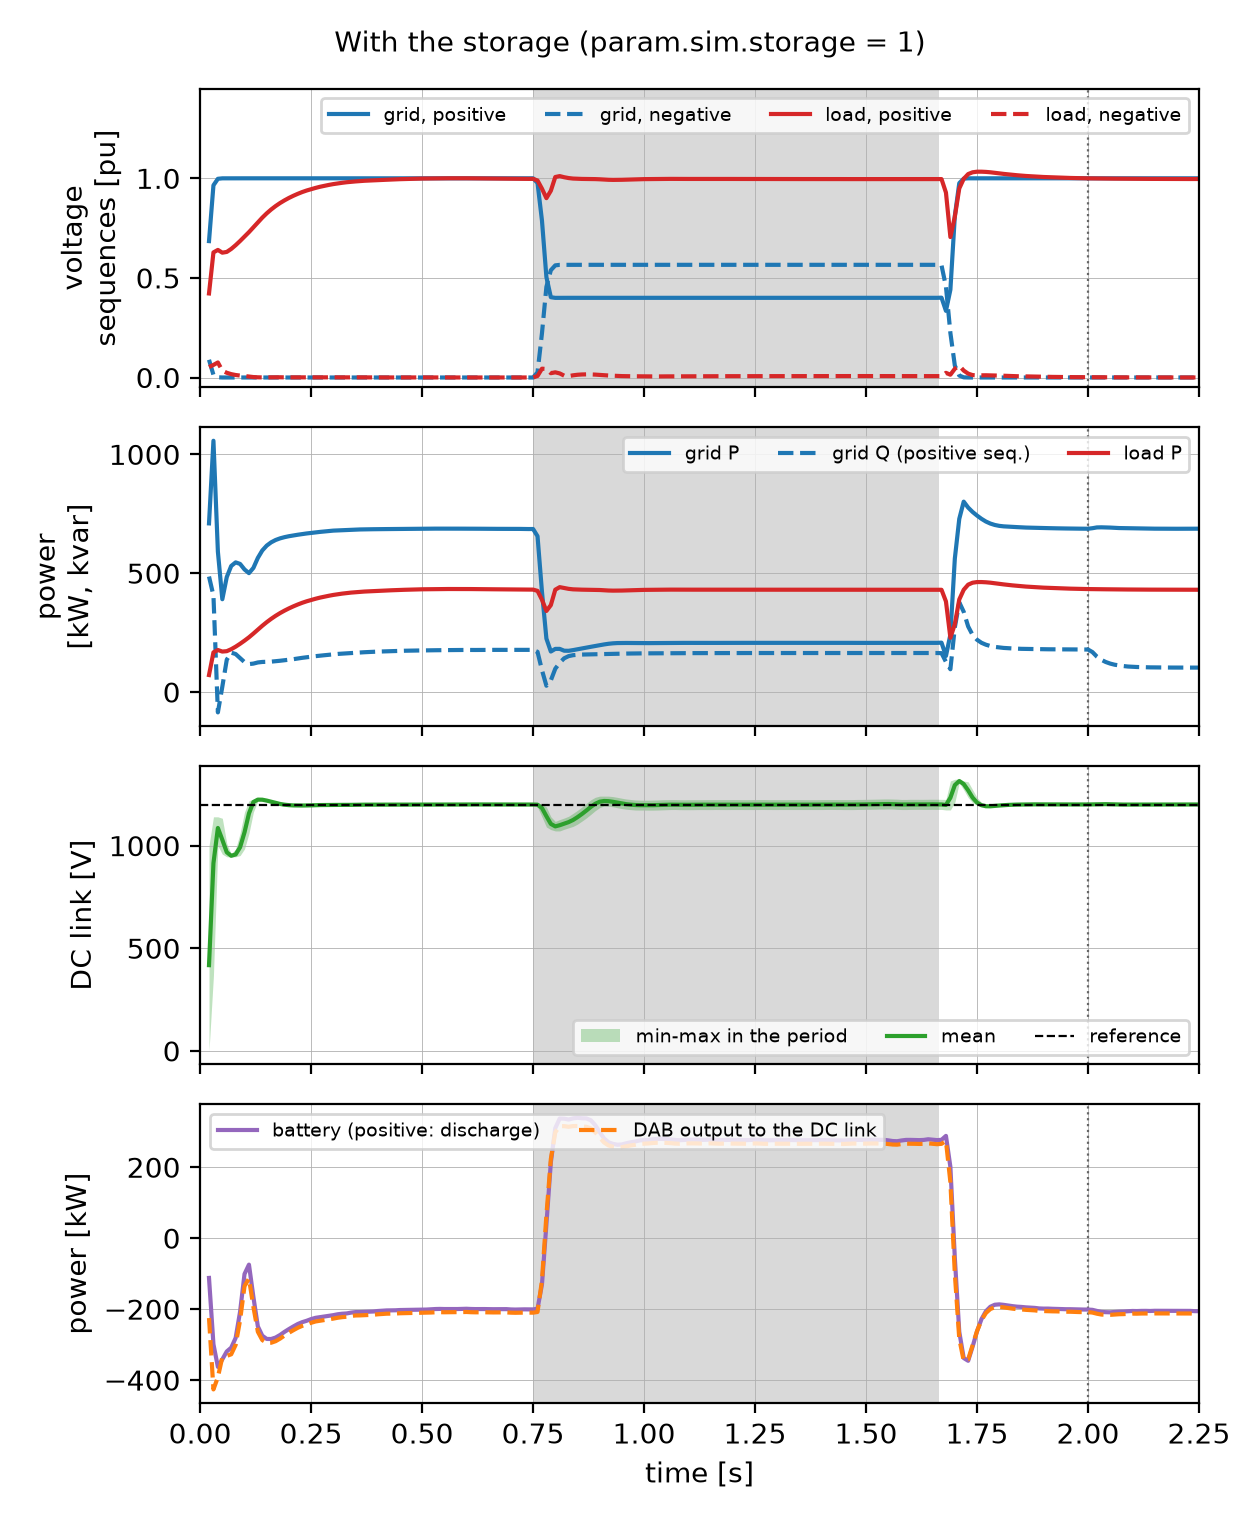
\includegraphics[width=0.86\textwidth]{figures/upqc_storage.png}
	\caption{Default case with the storage: sequence components of the grid and load voltages (pu of \SI{398}{V} phase rms), grid and load powers, DC-link voltage (mean, lowest and highest value over each grid period), battery and DAB power. Grey: the fault (test 25.4); dotted: the step of the reactive current.}
	\label{fig:res_storage}
\end{figure}

\begin{figure}[H]
	\centering
	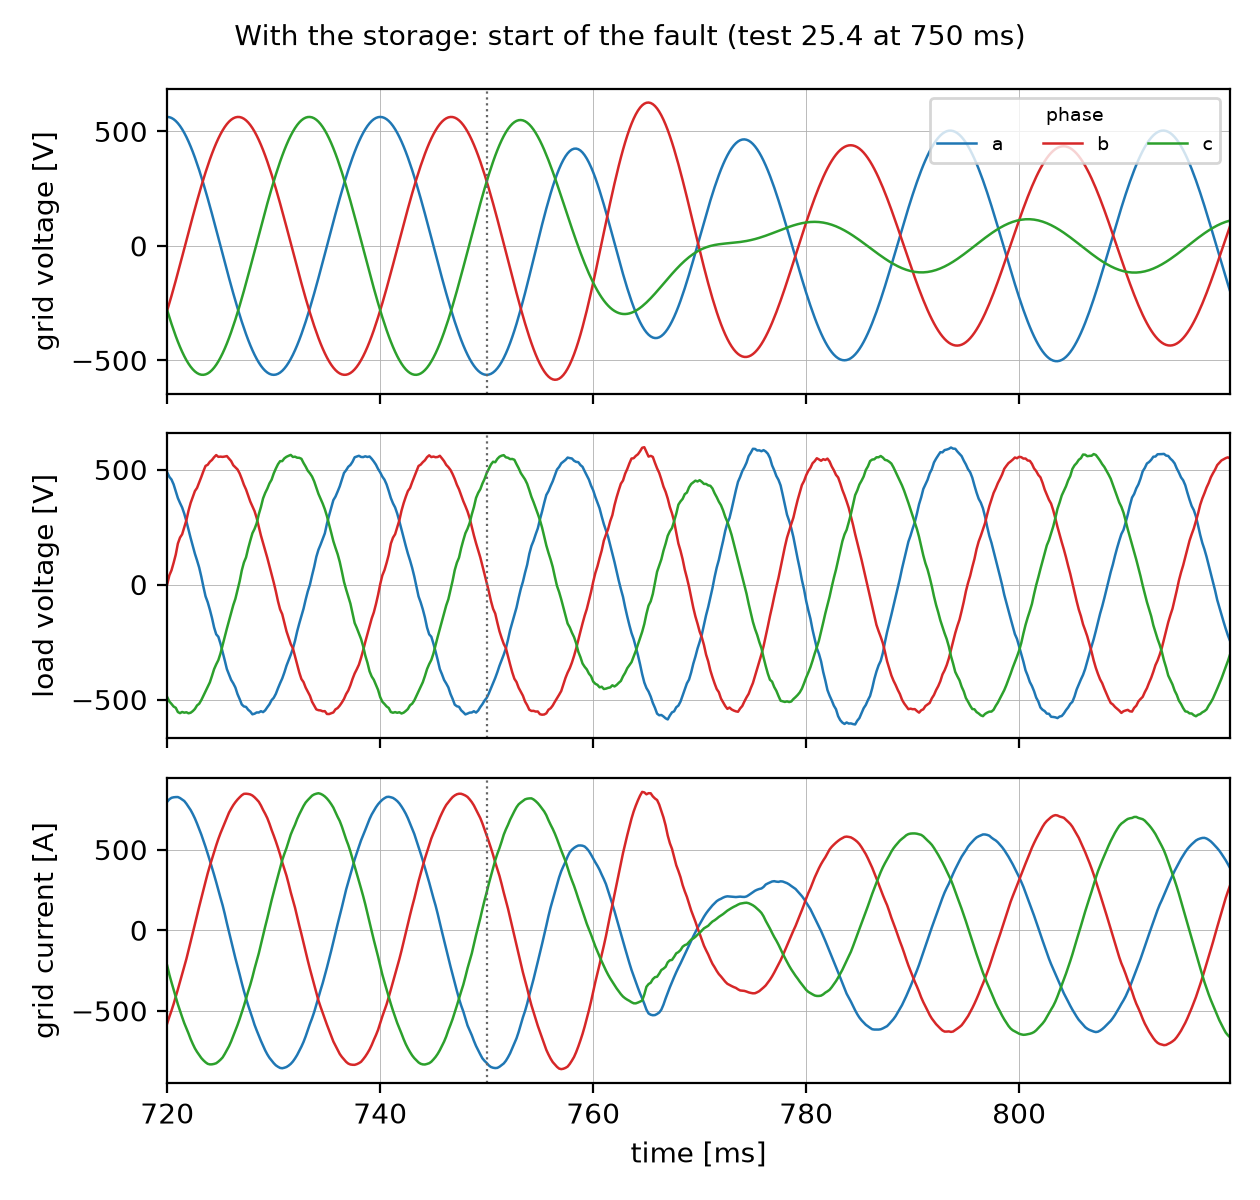
\includegraphics[width=0.86\textwidth]{figures/upqc_fault_onset.png}
	\caption{Default case with the storage: grid voltage, load voltage and grid current at the start of the fault.}
	\label{fig:res_onset}
\end{figure}

Figure~\ref{fig:res_dabfix} compares the default case with the DAB of \code{main} (phase shift up to $\pi$, PI gains $k\ped{p} = 1$, $k\ped{i} = \SI{35}{\per\second}$) and with the limit of the phase shift alone. With the DAB of \code{main} the DC link falls to \SI{0.5}{kV} within \SI{0.17}{s} of the start of the dip: the slow voltage PI winds up past the top of the power curve, the phase shift approaches $\pi$ and the power of the DAB collapses, then oscillates around \SI{150}{\kilo\watt} with the DC link between \SI{0.34}{kV} and \SI{0.87}{kV}; after the fault the DC link falls almost to zero and overshoots to \SI{2.25}{kV}, the SAF loses the control of its current (\SI{5.9}{kA} peak) and the system has not settled at \SI{2.25}{s}. With the limit and the gains of \code{main} the DAB stays at the top of its curve at the DC-link voltage of \SI{650}{V} (\SI{227}{\kilo\watt} from the battery, \SI{210}{\kilo\watt} into the DC link), and the DC link holds there through the fault; the recovery after the fault still takes the DC link to \SI{68}{V} and \SI{1.92}{kV} (SAF current \SI{4.8}{kA} peak). With the faster PI the DAB follows the step of power within a few tens of milliseconds and the DC link stays between \SI{1072}{V} and \SI{1323}{V} from the start of the dip to the end of the simulation.

\begin{figure}[H]
	\centering
	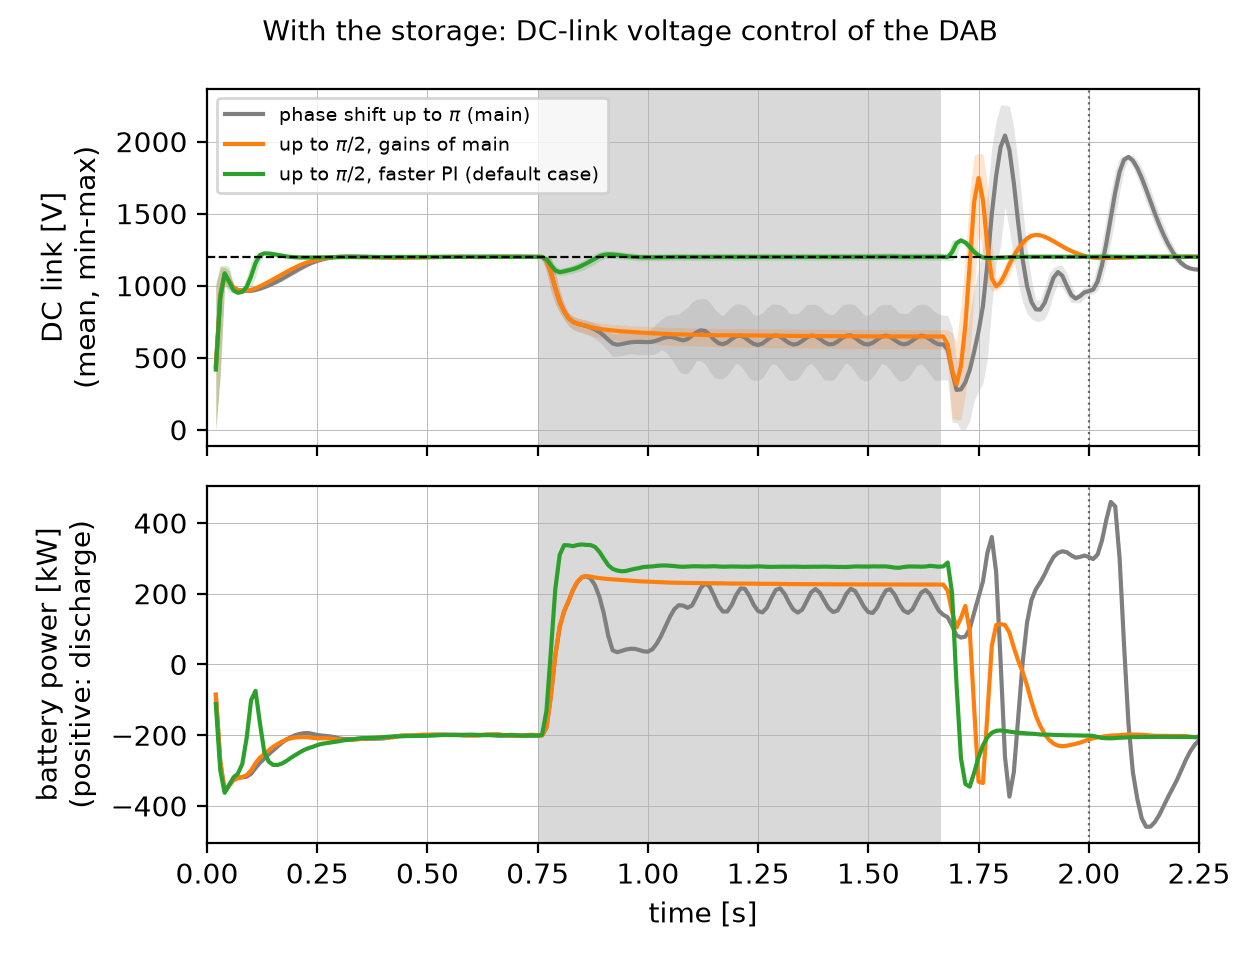
\includegraphics[width=0.86\textwidth]{figures/upqc_dab_fix.png}
	\caption{With the storage: DC-link voltage and battery power with the DAB of \code{main} (output of the voltage PI, the phase shift, limited to $\pm\pi$), with the limit $\pm\pi/2$ and the gains of \code{main}, and in the default case (limit $\pm\pi/2$, $k\ped{p} = 6$, $k\ped{i} = \SI{240}{\per\second}$).}
	\label{fig:res_dabfix}
\end{figure}

\subsection{Without the storage}
\label{sec:res_nostorage}

Figure~\ref{fig:res_nostorage} shows the case without the storage. Before the fault the SAF draws from the grid only the losses and the power of the VS: the grid gives \SI{464}{\kilo\watt} and \SI{169}{\kilo\var} for the \SI{432}{\kilo\watt} and \SI{136}{\kilo\var} of the load, the stack current of the SAF is \SI{37}{A} rms and the DC link stays at \SI{1200}{V} within \SI{\pm 1}{V}.

\begin{figure}[H]
	\centering
	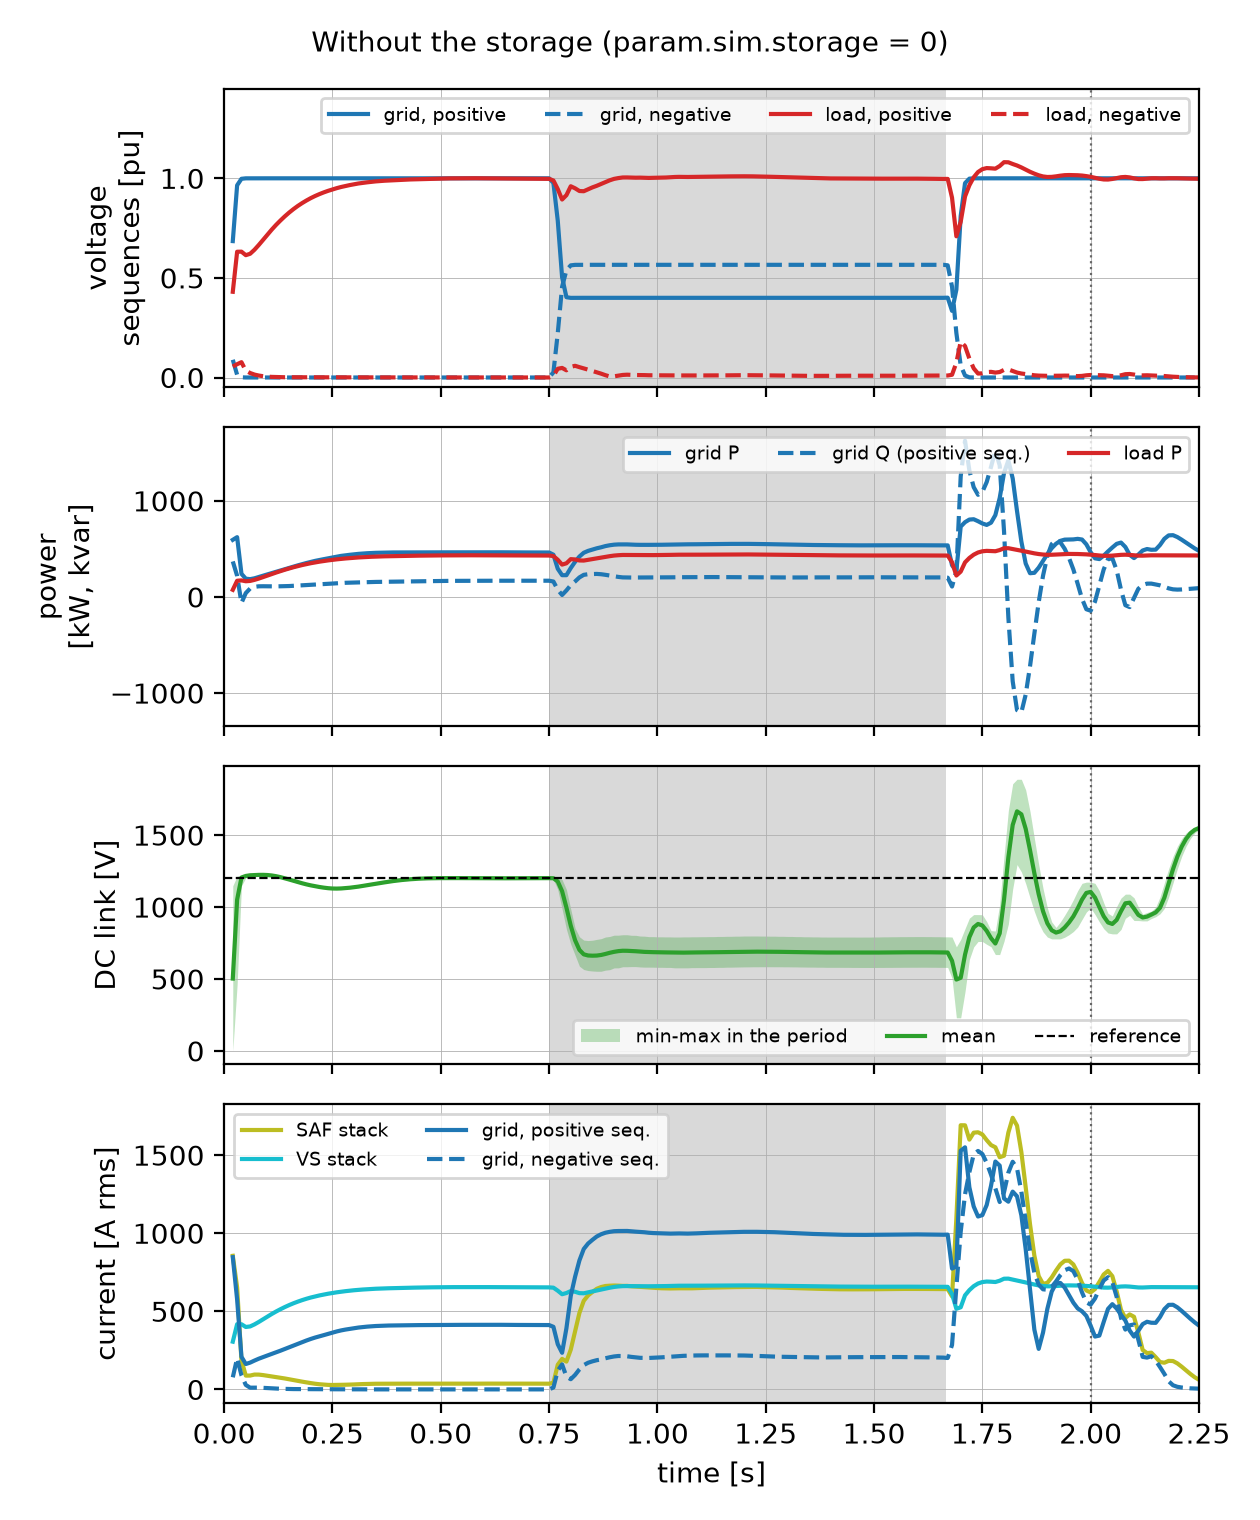
\includegraphics[width=0.86\textwidth]{figures/upqc_no_storage.png}
	\caption{Default case without the storage (\code{param.sim.storage = 0}): sequence components of the grid and load voltages, grid and load powers, DC-link voltage (mean, lowest and highest value over each grid period). Grey: the fault; dotted: the step of the reactive current.}
	\label{fig:res_nostorage}
\end{figure}

During the dip the VS keeps the load voltage (positive sequence \SI{399}{V}, \SI{1.00}{pu}; negative sequence \SI{3.7}{V}; THD \SI{4.5}{\percent}), but the SAF cannot bring from the faulted grid the power that the VS takes (Section~\ref{sec:res_energy}). The DC link falls to \SI{686}{V} on average (\SI{582}{V} to \SI{794}{V} within a period), below the peak of the line voltage of the faulted grid (more than \SI{850}{V} on the highest line voltage of this dip, \SI{976}{V} at the rated voltage): the bridge of the SAF conducts through its diodes, its current (\SI{646}{A} rms, 2.8 times $i\ped{s,nom}$) is no longer the one of its control, and the grid current has a negative sequence of \SI{208}{A}.

When the fault clears, the grid voltage passes through the same transition as with the storage while the DC link is low: the load voltage drops to \SI{0.71}{pu} (positive sequence \SI{282}{V} at \SI{1.69}{s}) with a negative sequence of up to \SI{72}{V} for about \SI{30}{ms}, then rises to \SI{1.08}{pu} (\SI{431}{V} at \SI{1.80}{s}). The grid charges the DC link through the diodes of the SAF and its filter: the DC link swings between \SI{0.23}{kV} (at \SI{1.69}{s}) and \SI{1.89}{kV} (at \SI{1.82}{s}), the SAF current reaches \SI{4.4}{kA} peak and the grid current stays unbalanced for about \SI{0.55}{s} (negative sequence below \SI{10}{A} from \SI{2.22}{s}). The DC link has not settled at the end of the simulation: at \SI{2.25}{s} it is at \SI{1.55}{kV} and rising, while the SAF draws less and less active current. The DC-link PI of the SAF, saturated for the whole fault, recovers slowly, and the slow oscillation of the DC link (period about \SI{0.2}{s}) shows a loop with little damping when the SAF current is limited. From \SI{1.74}{s} to the end the load voltage stays between \SI{0.99}{pu} and \SI{1.08}{pu} with a negative sequence below \SI{17}{V}.

The first version of the migration zeroed the active current of the SAF during the power limitation of the FRT also without the storage, as the block \code{udc\_ctrl} of \code{main} did. With it the DC link fell to \SI{602}{V}, the load voltage to \SI{0.97}{pu} with a negative sequence of \SI{14}{V} (THD \SI{8.9}{\percent}), and after the fault the DC link collapsed to almost zero and overshot to \SI{2.6}{kV}, with an overvoltage of \SI{1.18}{pu} and a negative sequence of \SI{106}{V} on the load for \SI{0.2}{s}. Hence the DC-link loop that stays active during the fault (Figure~\ref{fig:ixiref}).

\subsection{Currents}
\label{sec:res_currents}

Figure~\ref{fig:res_currents} gives the rms currents over each grid period, divided by the rated current $i\ped{s,nom} = \SI{232}{A}$ of the \SI{250}{\kilo\watt} data set of SAF and VS. The VS carries the load current through the series transformer, \SI{654}{A} rms in every part of the test, 2.8 times its rated current (Section~\ref{sec:oppoint}). The stack current of the SAF is \SI{214}{A} rms with the storage before the fault (its constant active current) and \SI{251}{A} during the dip (the reactive currents of the FRT); without the storage it is \SI{37}{A} before the fault and \SI{646}{A} during the dip, when its bridge conducts through the diodes.

\begin{figure}[H]
	\centering
	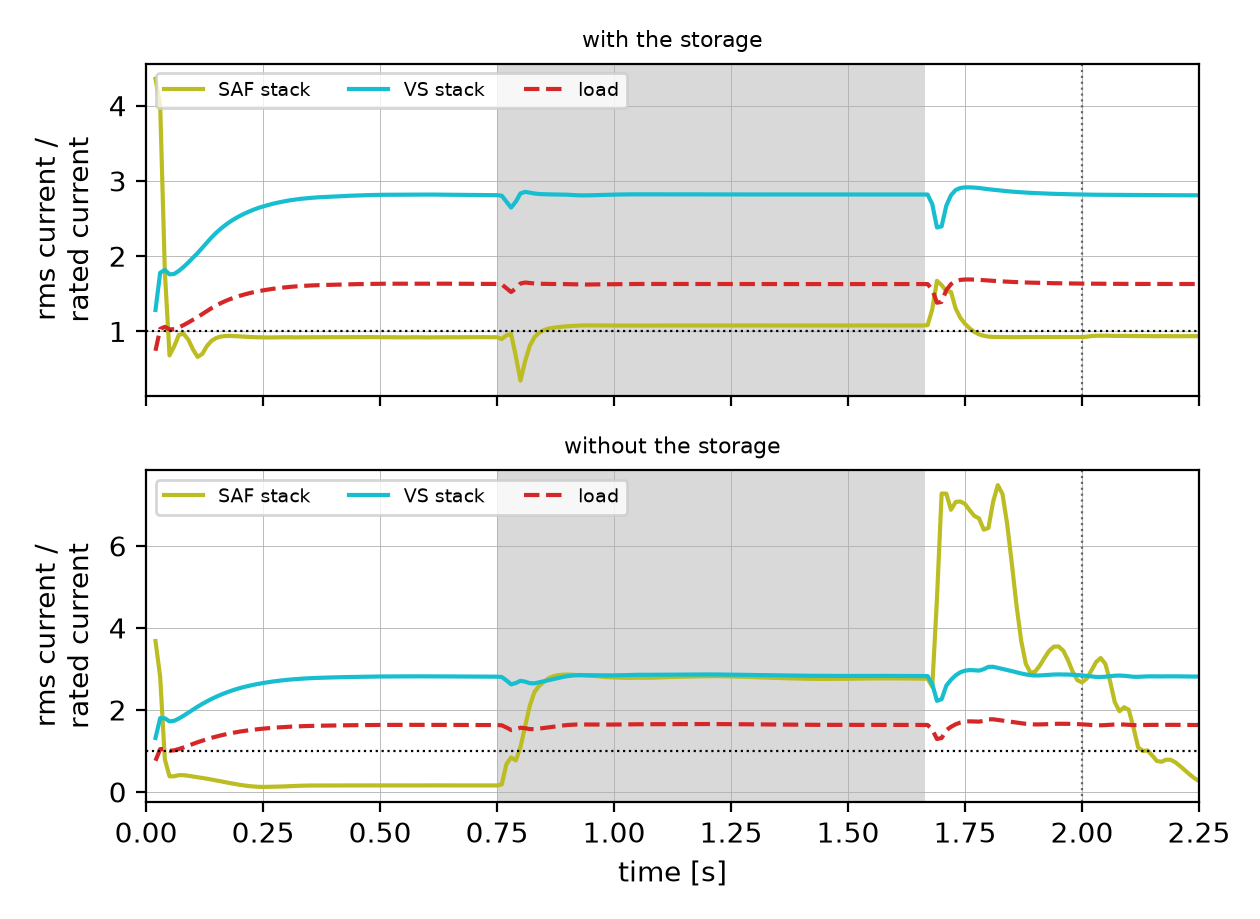
\includegraphics[width=0.86\textwidth]{figures/upqc_currents.png}
	\caption{Rms stack currents of SAF and VS and load current over each grid period, divided by the rated current of the data set of SAF and VS (\SI{232}{A}), with and without the storage.}
	\label{fig:res_currents}
\end{figure}

% =============================================================
\section{Changes of November 2026}
\label{sec:changes}

The model of the branch \code{main} worked with the full licence. The branch \code{dev} had removed blocks to stay within the Home licence, but its init no longer ran with the library and the model had broken links. The revision (pull request \#1 of the repository, towards \code{dev}) did the following.

\paragraph{Init.} \code{init\_model.m} rewritten as one \code{param} struct with the local functions of \code{private/}, which replace the setup functions of the library with the same formulas (\code{timing\_setup}, \code{grid\_three\_phase\_emulator}, \code{frt\_settings}, \code{three\_phase\_afe\_hwdata}, \code{ctrl\_afe\_setup}, \code{three\_phase\_transformer\_setup}, \code{single\_phase\_dab\_hwdata}, \code{lithium\_ion\_battery\_setup}); the checks of the model at the end; the legacy init kept as \code{init\_model\_legacy.m}. Fixes on the way: the magnetizing current of the delta winding of the grid transformer (three times the value of the legacy formula), the data set \code{DAB\_800V}, the test 25.3 of the FRT catalogue (not defined). The fixes of the library functions are in pull request \#38 of \code{pwr-control/library}.

\paragraph{Model.}
\begin{itemize}[nosep]
	\item \emph{DAB that transferred no power.} The ideal bridges of \code{ideal\_bridges\_lib} have integrated passives on by default: \SI{0.5}{mH} in series with each AC terminal of a full bridge, \SI{1}{mH} per phase of a three-phase bridge and \SI{2}{mF} on the DC side of each bridge, on top of the filters, DC links and transformer of the model. The series inductance of the DAB became about \SI{2}{mH} (\SI{1}{mH} per bridge) instead of \SI{38}{\micro\henry}, and the DAB could not deliver its power. They are off in the four bridges.
	\item \emph{Phase shift of the DAB beyond the top of the power curve.} The DC-link voltage PI of the DAB gives the phase shift directly, with its output limited to $\pm 2$ times $\pi/2$: limit $\pm 1$, \code{param.dab.ctrl.phase\_lim} (Section~\ref{sec:dab}).
	\item \emph{Start-up} from the initial conditions, with the battery at its OCV (Section~\ref{sec:startup}).
	\item \emph{DC-link voltage loop of the SAF} (commented out in \code{main}, removed in \code{dev}) back, for the case without the storage, with the switch of Figure~\ref{fig:ixiref}.
	\item \emph{Load voltage of the VS.} Its sequences read the tag \code{ugd\_abc\_pu}, a voltage of the SAF that the VS cannot see; they read \code{ugd\_abc\_load\_pu}.
	\item \emph{Readers of the removed blocks} (Section~\ref{sec:licence}) deleted: scopes and logging of the power meter, of the instantaneous power and of the device quantities of the DAB; the logging buses of SAF and VS rebuilt with the signals that exist; the modulators take $u_{\alpha\beta\gamma}$ as a vector, as \code{current\_ctrl\_uvw} gives it; the clock of the DAB without alignment.
	\item \emph{Names.} Labels with \code{saf}, \code{vs}, \code{dab} (for example \code{left\_shunt\_universal\_power\_\allowbreak quality\_compensator} $\to$ \code{upqc}, \code{shunt\_active\_filter} $\to$ \code{saf}, \code{voltage\_stabiliser} $\to$ \code{vs}, \code{dab\_mod1} $\to$ \code{dab}); tags, To Workspace variables and block parameters on the names of \code{param}; the model configuration reads \code{param.sim.simlength} and \code{param.glb\_time.tc}. The README of the folder has the complete tables of the old and new names.
\end{itemize}

The changes to the model are made by a script, \code{ls\_upqc/migration/ls\_upqc\_migrate.m}, applied once to the model of \code{dev} with the model of \code{main} as the source of the restored blocks: it is the readable record of what changed in the binary \code{.slx} file, and it can be applied again to a newer \code{dev} model.

% =============================================================
\section{Open points}
\label{sec:open}

\begin{enumerate}
	\item \textbf{Rating of the VS and of the series transformer.} With the default load the VS carries \SI{654}{A} rms, 2.8 times the rated current of its data set, and the line windings of the series transformer \SI{380}{A} against their \SI{181}{A} (Section~\ref{sec:oppoint}). The ideal switches do not mind, but the case is not a realistic sizing: a smaller load (for example \SI{150}{\kilo\watt}, within the rating of the VS) or a series transformer rated for the load current would make the currents of Figure~\ref{fig:res_currents} meaningful.
	\item \textbf{Deep asymmetric dip without the storage.} At \SI{0.40}{pu} of positive sequence the SAF, limited to \SI{1.65}{pu} of active current, cannot bring from the grid the power that the VS needs to hold the load voltage of the default load (Section~\ref{sec:res_nostorage}): the DC link falls below the peak line voltage and the SAF loses the control of its current until the end of the transient. The case without the storage needs a milder test (a dip of \SI{25}{\percent}, tests 75.1 to 75.8 of the catalogue), a smaller load or a higher current limit of the SAF.
	\item \textbf{DAB without current loop and without series capacitor.} The current PI of the DAB (block \code{i\_out\_ctrl}) is commented out, as in \code{main}, so the battery current is neither controlled nor limited: the battery gives \SI{276}{\kilo\watt} during the dip of the default test, 1.1 times its rated power, and takes \SI{346}{\kilo\watt} for a moment after it. A current loop under the voltage loop, with its limit, would protect the battery and the bridges. The transformer has no series capacitor (Section~\ref{sec:dab}), so nothing blocks a DC component of its current; a real DAB needs a blocking capacitor or a control of the flux balance.
	\item \textbf{No protection of the DC link and of the SAF current.} When the DC link is below the peak line voltage the SAF current is limited only by the grid impedance and the filter (\SI{4.4}{kA} peak without the storage); a real converter would trip. An undervoltage limit that blocks or limits the VS before the DC link falls below the peak line voltage, and a peak current protection of both bridges, are missing from the model.
	\item \textbf{Start-up without precharge.} The DC link is charged through the diodes of the SAF from zero, with a grid current of \SI{2.3}{kA} peak in the first period. A precharge resistor, or an initial DC-link voltage, would give a cleaner start.
	\item \textbf{Battery and DAB sizing.} The battery (\SI{50}{Ah}) is charged at about \SI{3}{C} in normal operation; its RC branch has a time constant of \SI{0.72}{ms}, a consequence of the scaling of the legacy init (Section~\ref{sec:oppoint}).
	\item \textbf{Step of the DAB.} $t\ped{s,DAB}/t\ped{c} = 66.7$ is not an integer (Section~\ref{sec:timing}): a base step of $t\ped{s,SAF}/300$ would fix it at 1.5 times the simulation time.
	\item \textbf{Release of the FRT power limitation.} The block \code{frt\_vde4110} of \code{afe\_uvw\_ctrl} releases the limitation when the negative sequence is below \SI{0.7}{pu}, probably a slip for \SI{0.1}{pu} minus the hysteresis (note \cite{afe_uvw_note}): with the default test it has no effect, since the positive sequence keeps the limitation on.
	\item \textbf{Post-processing scripts.} \code{video\_plot\_sim.m} reads \path{..\sim_results_icc20inom_3.mat} with a window from \SI{1.95}{s} to \SI{3.00}{s}, and two scripts of \path{video_plots/} read \code{sim\_results\_1.mat}: results of longer simulations of the legacy init. The file and the time windows must be set for the results at hand.
	\item \textbf{Future changes of the model of \code{dev}.} The migration script runs on the model of \code{dev} before the migration; a change made on a newer \code{dev} model must be made on the migrated one by hand (or the script adapted).
\end{enumerate}

% =============================================================
\appendix
\section{Files}
\label{sec:files}

\begin{table}[H]
	\centering
	\captionsetup{width=0.9\textwidth, font=small}
	\caption{Files referred to in this note.}
	\label{tab:files}
	\rowcolors{2}{tableShade}{white}
	\small
	\begin{tabularx}{0.97\textwidth}{@{} >{\raggedright\arraybackslash}p{0.38\textwidth} X @{}}
		\toprule
		\textbf{File} & \textbf{Content} \\
		\midrule
		\multicolumn{2}{@{}p{\dimexpr0.97\textwidth-2\tabcolsep\relax}@{}}{\textbf{\code{left-shunt-unified-power-quality-conditioner}, folder \path{ls_upqc/}}} \\
		\code{init\_model.m} & initialization (live script in plain-text format), one \code{param} struct \\
		\code{ls\_upqc.slx} & the model \\
		\code{ls\_upqc\_private.m}, \path{private/} & handles to the local functions of the init; the functions \\
		\code{plot\_sim.m}, \code{plot\_spectrum.m} & figures of a simulation; spectrum of the grid voltage \\
		\code{video\_plot\_sim.m}, \path{video_plots/} & MP4 animations \\
		\code{iec\_power\_meter.m} & sequence powers from logged waveforms \\
		\code{results\_compat.m} & names of the new init for the results of the legacy init \\
		\code{non\_virtual\_blocks\_counting.m} & count of the nonvirtual blocks \\
		\path{migration/ls_upqc_migrate.m} & the changes of November 2026 to the model, as a script \\
		\code{init\_model\_legacy.m} & the legacy init, for reference \\
		\code{README.md} & user guide and tables of the old and new names \\
		\midrule
		\multicolumn{2}{@{}p{\dimexpr0.97\textwidth-2\tabcolsep\relax}@{}}{\textbf{\code{repositories-documentation}, folder \path{repos_doc/unified_power_quality_conditioner/}}} \\
		\code{upqc.tex}, \code{upqc.pdf} & this note \\
		\path{py/upqc_summary.m} & MATLAB: summary of a simulation (one row every \SI{10}{ms}, waveforms of the fault onset, numbers) \\
		\path{py/upqc_figures.py} & Python: the figures of Section~\ref{sec:results} from the summaries \\
		\path{py/data/} & the summaries of the two simulations of Section~\ref{sec:results} \\
		\bottomrule
	\end{tabularx}
	\rowcolors{1}{white}{white}
\end{table}

% =============================================================
\begin{thebibliography}{99}
	\small
	\bibitem{fujita1998} H.~Fujita and H.~Akagi, ``The unified power quality conditioner: the integration of series- and shunt-active filters,'' \emph{IEEE Trans. Power Electron.}, vol.~13, no.~2, pp.~315--322, Mar. 1998.
	\bibitem{khadkikar2012} V.~Khadkikar, ``Enhancing electric power quality using UPQC: a comprehensive overview,'' \emph{IEEE Trans. Power Electron.}, vol.~27, no.~5, pp.~2284--2297, May 2012.
	\bibitem{pcim_paper} D.~Bagnara, ``A flipped unified power quality conditioner for active distribution networks: topology, modelling, and control strategy,'' paper prepared for PCIM, folder \path{doc/} of \code{pwr-control/left-shunt-unified-power-quality-conditioner}.
	\bibitem{vde4110} VDE-AR-N 4110, \emph{Technical requirements for the connection and operation of customer installations to the medium voltage network (TAR medium voltage)}, VDE, 2018.
	\bibitem{dedoncker1991} R.~W.~A.~A. De Doncker, D.~M. Divan, and M.~H. Kheraluwala, ``A three-phase soft-switched high-power-density dc/dc converter for high-power applications,'' \emph{IEEE Trans. Ind. Appl.}, vol.~27, no.~1, pp.~63--73, Jan./Feb. 1991.
	\bibitem{iec61000430} IEC 61000-4-30, \emph{Electromagnetic compatibility (EMC) -- Part 4-30: Testing and measurement techniques -- Power quality measurement methods}, IEC, 2015.
	\bibitem{ieee1459} IEEE Std 1459-2010, \emph{IEEE standard definitions for the measurement of electric power quantities under sinusoidal, nonsinusoidal, balanced, or unbalanced conditions}, IEEE, 2010.
	\bibitem{afe_uvw_note} D.~Bagnara, \emph{AFE control in the uvw frame: the five MATLAB Function blocks of \code{afe\_uvw\_ctrl}}, technical note, rev.~01, Nov. 2026, \path{repos_doc/afe_uvw_ctrl} of \code{pwr-control/repositories-documentation}.
	\bibitem{library} \code{pwr-control/library}, branch \code{dev}: masked models, setup functions and C sources of the pwr-control models, \url{https://github.com/pwr-control/library}.
\end{thebibliography}

\end{onehalfspace}
\end{document}
